% !TEX root = INT.tex

\chapter{Signal Region Definition}
\label{chap:SignalRegion}

\indent The kinematic selections in the signal region are designed to maximize signal acceptance and reject SM $\ttbar$ events.  SM $\ttbar$ is the dominant background for this analysis and comprises $70$\% of backgrounds in the signal region.  The signal region selections are also effective at rejecting subdominant backgrounds, including $W$+jets, single top, $Z$+jets and QCD multijet backgrounds.  \\

\indent This chapter first builds physical intuition on the dominant SM $\ttbar$ in section \ref{sec:SR:physical} and explains how the signal region selections reject background.  The signal region kinematic selections are defined in section \ref{sec:SR:Selections}.  A back-of-the-envelope estimation of the signal region background rejection power and an order-of-magnitude estimation of how the signal over background ratio improves with the signal region selections is given in section \ref{sec:SR:estimate}. Lastly, the signal region yields and background composition are covered in sections \ref{sec:SR:Yields} and \ref{sec:Bkg:Compositiion}.  \\

\section{Physical Intuition on how Signal Region Selections Reject Background}
\label{sec:SR:physical}

\indent The zero-lepton signal region is designed specifically to reject the dominant $\ttbar$ background while maximizing signal acceptance.  The signal region design and the signal and $\ttbar$ kinematics are summarized in this section.  The signal region selections' effects on subdominant backgrounds are also described near the end of the section. More detail on each SM background, including background estimation techniques, can be found in chapter \ref{chap:backgrounds}. \\

\indent  We find that 95\% of all $\ttbar$ which survive the signal region selections decay via the single hadronic tau, single electron, or single muon decay channels.  SM $\ttbar$ that decays via the fully hadronic decay channel generates little intrinsic $\MET$ and is negligible in the signal region.  The SM $\ttbar$ dileptonic decay branching ratio is a factor of 5 lower than the single lepton decay channel. Plus, di-leptonic $\ttbar$ has a higher probability of being rejected by the lepton veto.  A pie chart of the branching fractions for different $\ttbar$ decay channels is shown in Figure \ref{fig:ttbardecay}. \\

\begin{figure}[h!]
  \begin{center}
    	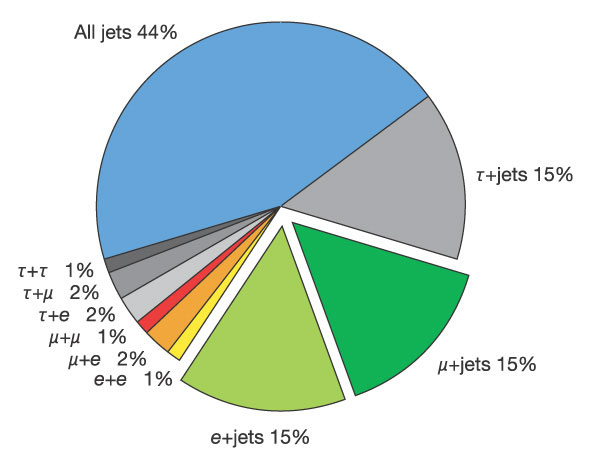
\includegraphics[width=0.85\textwidth]{figures/strategy/ttbarDecay.jpg}
   \end{center}
\caption{ Pie chart of the branching fractions for different $\ttbar$ decay channels. }
\label{fig:ttbardecay} 
\end{figure}

\indent The $\met$ and $\RISR = \met/\PTISR$ distributions after the zero-lepton preselection for stop signal and SM backgrounds can be seen in Figure \ref{fig:presel_dist_1} and \ref{fig:presel_dist_2}.  \\

\begin{figure}[h!]
\centering
    	 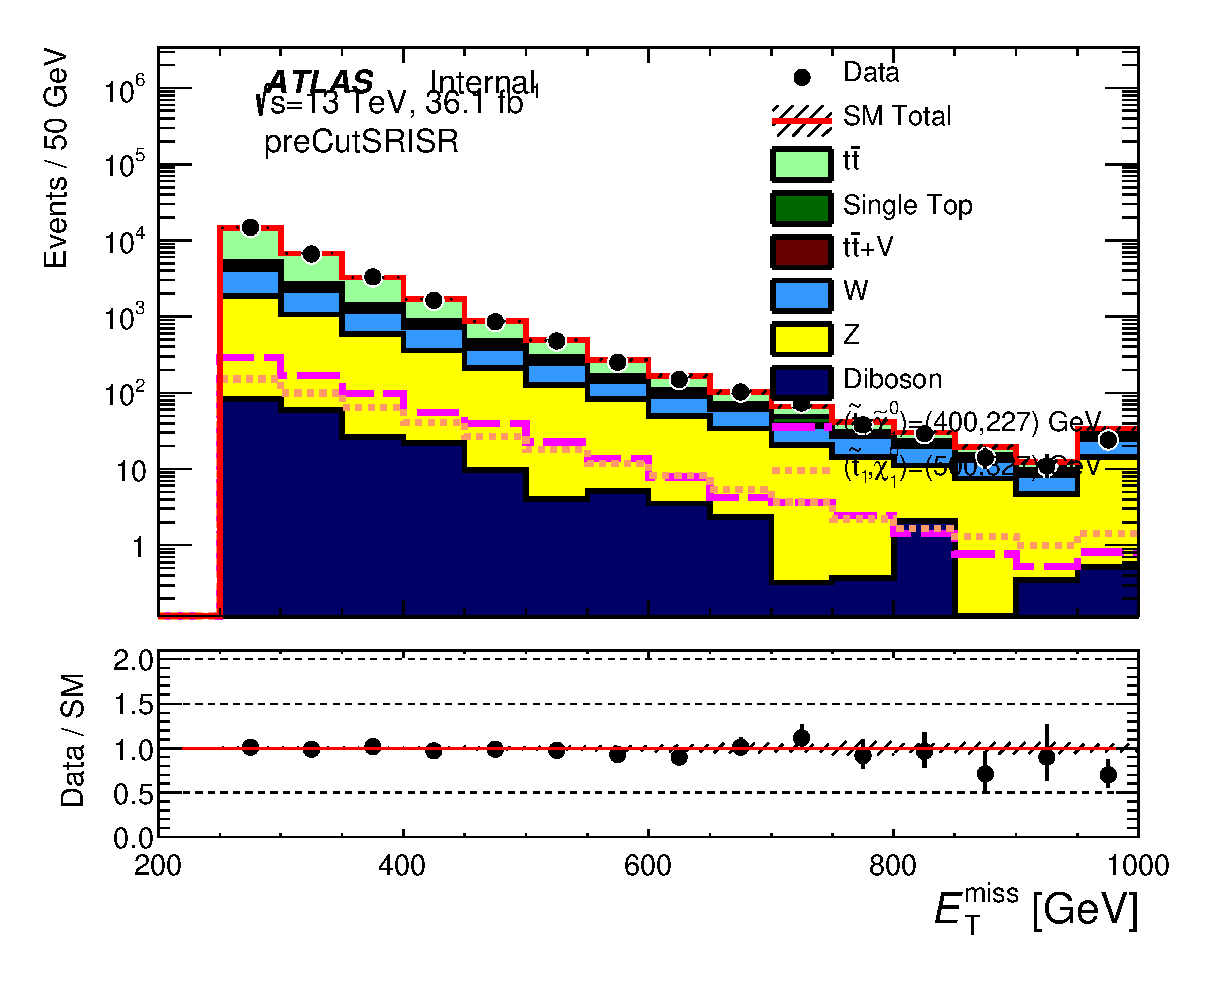
\includegraphics[width=0.85\textwidth]{figures/plotRegion/Met_preCutSRISR_log.eps}
\caption[The $\met$ distribution after zero-lepton preselection for stop signal and SM background]{ The $\met$ distributions after the zero-lepton preselection.  SM backgrounds are displayed as the solid stacked histograms.  Stop signals with$(m_{\stop}, m_{\ninoone}) = (400 \gev,227 \gev)$ and $(500 \gev, 327 \gev)$ are shown as dashed histograms.  } %Signal strength is increased by a factor of 20 for better visibility. }
\label{fig:presel_dist_1} 
\end{figure}

\begin{figure}[h!]
  \centering
	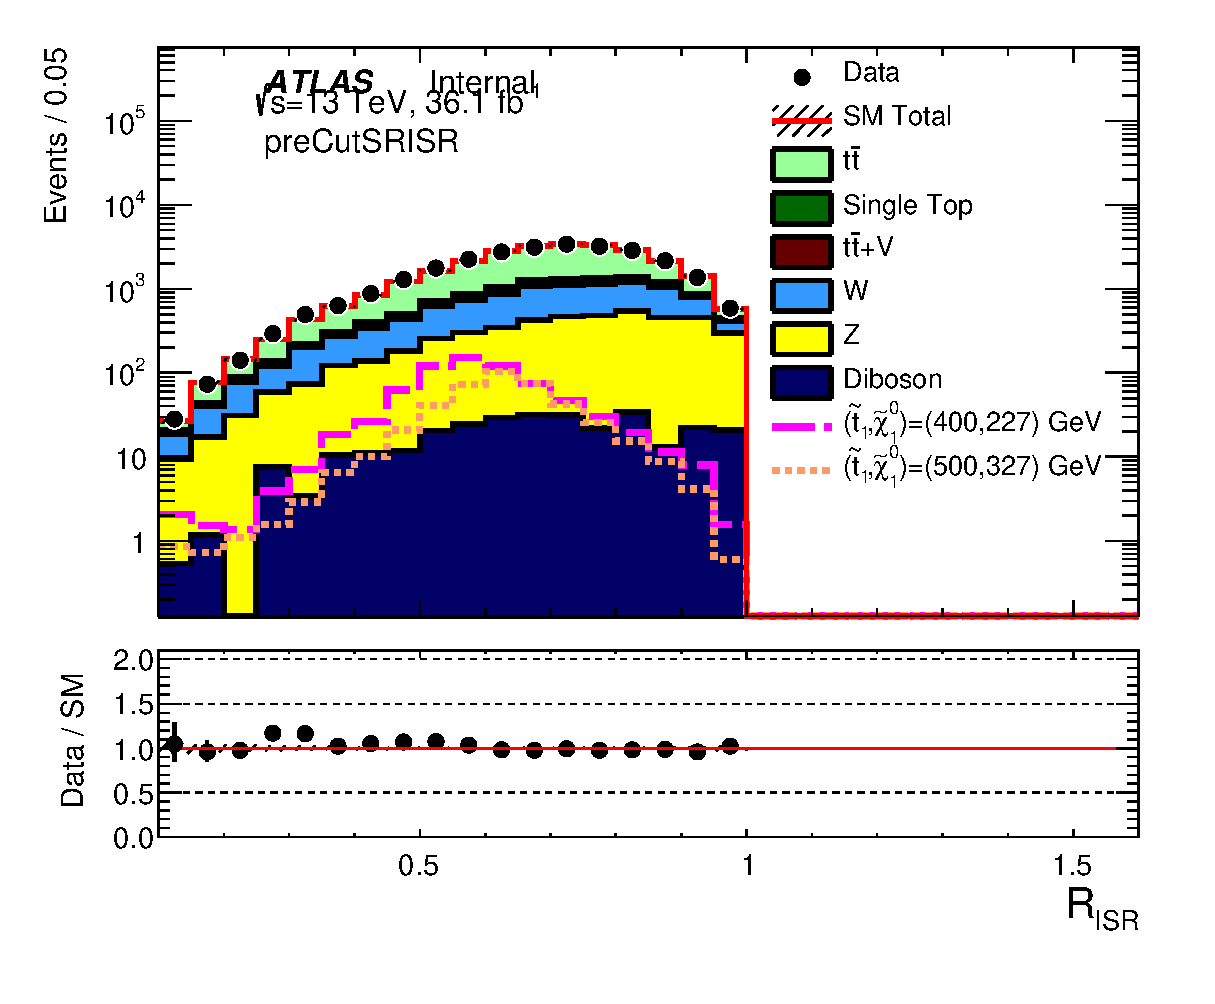
\includegraphics[width=0.85\textwidth]{figures/plotRegion/CA_RISR_preCutSRISR_log.eps}
\caption[The $\RISR = \met/\PTISR$ distribution after zero-lepton preselection for stop signal and SM background]{ The $\RISR$ distribution after preselection.  SM backgrounds are displayed as the solid stacked histograms.  Stop signals with $(m_{\stop}, m_{\ninoone}) = (400 \gev,227 \gev)$ and $(500 \gev, 327 \gev)$ are shown as dashed histograms. } % Signal strength is increased by a factor of 20 for better visibility. }
\label{fig:presel_dist_2} 
\end{figure}

\indent  The $\met$ distribution is very similar between stop signal and SM background, but the signal peaks in the $\RISR$ distribution.  The $\RISR$ peak in signal is wide because we have not made a requirement for high ISR $\pt$ at the preselection level.  This signal peak will sharpen with the additional signal region selections.  \\

\indent The $\ttbar$ $\RISR$ distribution peaks at $\sim0.75$.  This corresponds to $\ttbar$ events without hard ISR which gives a high $\met/\PTISR$ ratio.  Again, no requirement on $\PTISR$ has been made at the preselection level.  After placing more signal region requirements on events with high ISR $\pt$,  the $\ttbar$ events with high $\RISR$ ratio will be rejected.  The rest of this section will be devoted to explaining why the $\ttbar$ background initially peaks at $\sim0.75$ and how the signal region selections reject these high $\RISR$ $\ttbar$ events.  \\

\indent First, it is important to note that the top decay cannot generate a 250 $\gev$ $\pt$ neutrino if the top decays at rest.  Therefore, the $\MET > 250 \gev$ requirement in preselection selects mainly for $\ttbar$ with a boosted leptonic top.   \\

\indent  The leptonic top can only gain boost in one of two ways.  Either the leptonic top recoils against the hadronic top in a back-to-back fashion, or both tops recoil against hard ISR.  This break-down of SM $\ttbar$ into two kinematically distinct populations is covered in more detail in section \ref{sec:Bkg:ttbar}.  A schematic representation of these two distinct $\ttbar$ kinematic populations can be found in Figure \ref{fig:ttbar:2pop}. \\

\begin{figure}[h!]
  \centering
	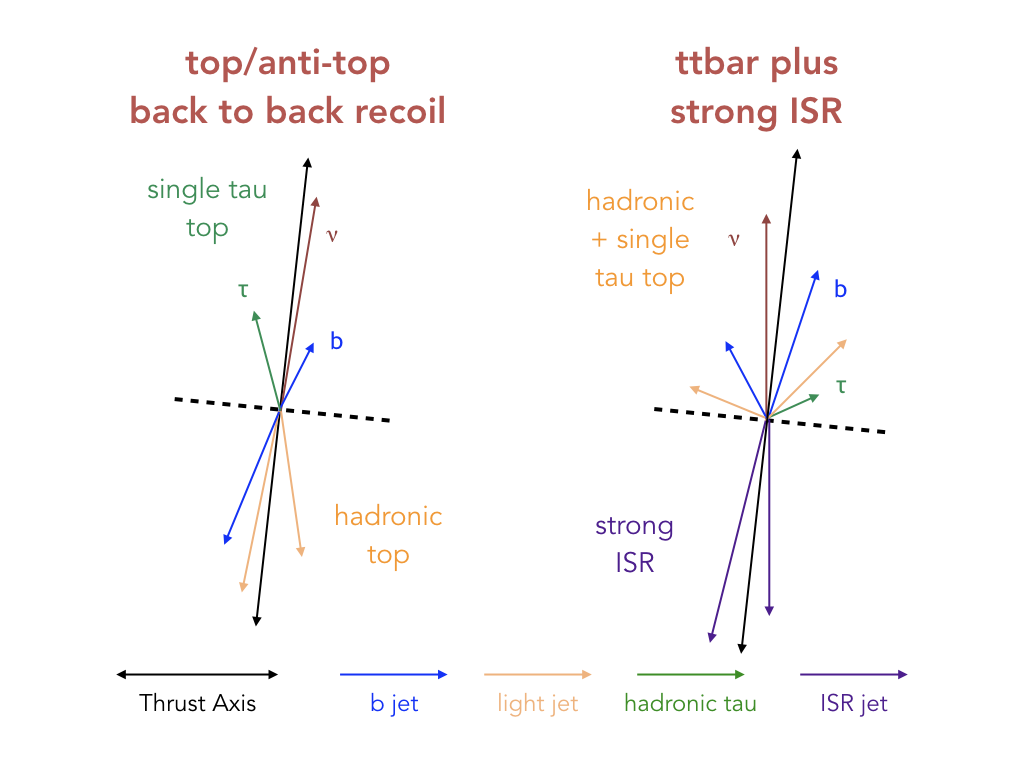
\includegraphics[width=0.85\textwidth]{./figures/strategy/ttbar_2pop.png}
	\caption[Schematic depiction of the kinematics of the $\ttbar$ back-to-back $\ttbar$ population and the $\ttbar$+hard ISR population that exists after the zero-lepton pre-selection.]{Depiction of the kinematics of the $\ttbar$ back-to-back population and the $\ttbar$+hard ISR population that exists after the zero-lepton pre-selection. The two example events' thrust axis are aligned.  The hemisphere containing $\met$ has significantly higher jet multiplicities and total energy in $\ttbar$+hard ISR events. }
\label{fig:ttbar:2pop}
\end{figure}

\indent The thrust axis or the axis that maximizes the amount of back-to-back $\pt$ along it contains important information in both populations.  In the $\ttbar$ back-to-back population, the thrust axis aligns along the top/anti-top back-to-back boost.  In the $\ttbar$+hard ISR population, the thrust axis aligns along the ISR/$\ttbar$ back-to-back boost.  \\

\indent  After preselection, 90\% of all $\ttbar$ events belong to the $\ttbar$ back-to-back population.  Boosting one top against the other top simply requires less center-of-mass energy than boosting both tops with additional hard ISR.  \\

\indent In the $\ttbar$ back-to-back population, the hadronic top's decay products will be mainly in the hemisphere not containing $\met$.  The reconstructed ISR $\pt$ will therefore be approximately the hadronic top $\pt$.  The leptonic top and hadronic top have roughly equal $\pt$ because the two tops are back-to-back.  The leptonic top will have its $\pt$ split between its decay products.  For this reason, we would expect the $\RISR$ to be approximately 1/3 as the neutrino would be expected to carry about 1/3 the leptonic top $\pt$ if no selections were applied. Some $\ttbar$ events will have a high $\RISR$ ratio because the neutrino carries a higher fraction of the leptonic top $\pt$ because of specific alignments between the top boost and the decay axes. \\

\indent However, the $\ttbar$ differential cross section as a function of $m^{t\tbar}$, shown in Figure \ref{fig:ttbar:mtt}, falls exponentially.  $m^{t\tbar}$ is directly related to the amount of back-to-back boost between the two tops and the $\pt$ of each top.  After the $\met > 250 \gev$ requirement, most $\ttbar$ events have a low $m^{t\tbar}$ but the neutrino receives a large fraction of the top $\pt$ instead of having a high $m^{t\tbar}$ and the neutrino receiving a small fraction of the top $\pt$.  This leads to a higher $\RISR$ peak at $\sim0.75$ for the $\ttbar$ back-to-back population. \\

\begin{figure}[h!]
  \centering
	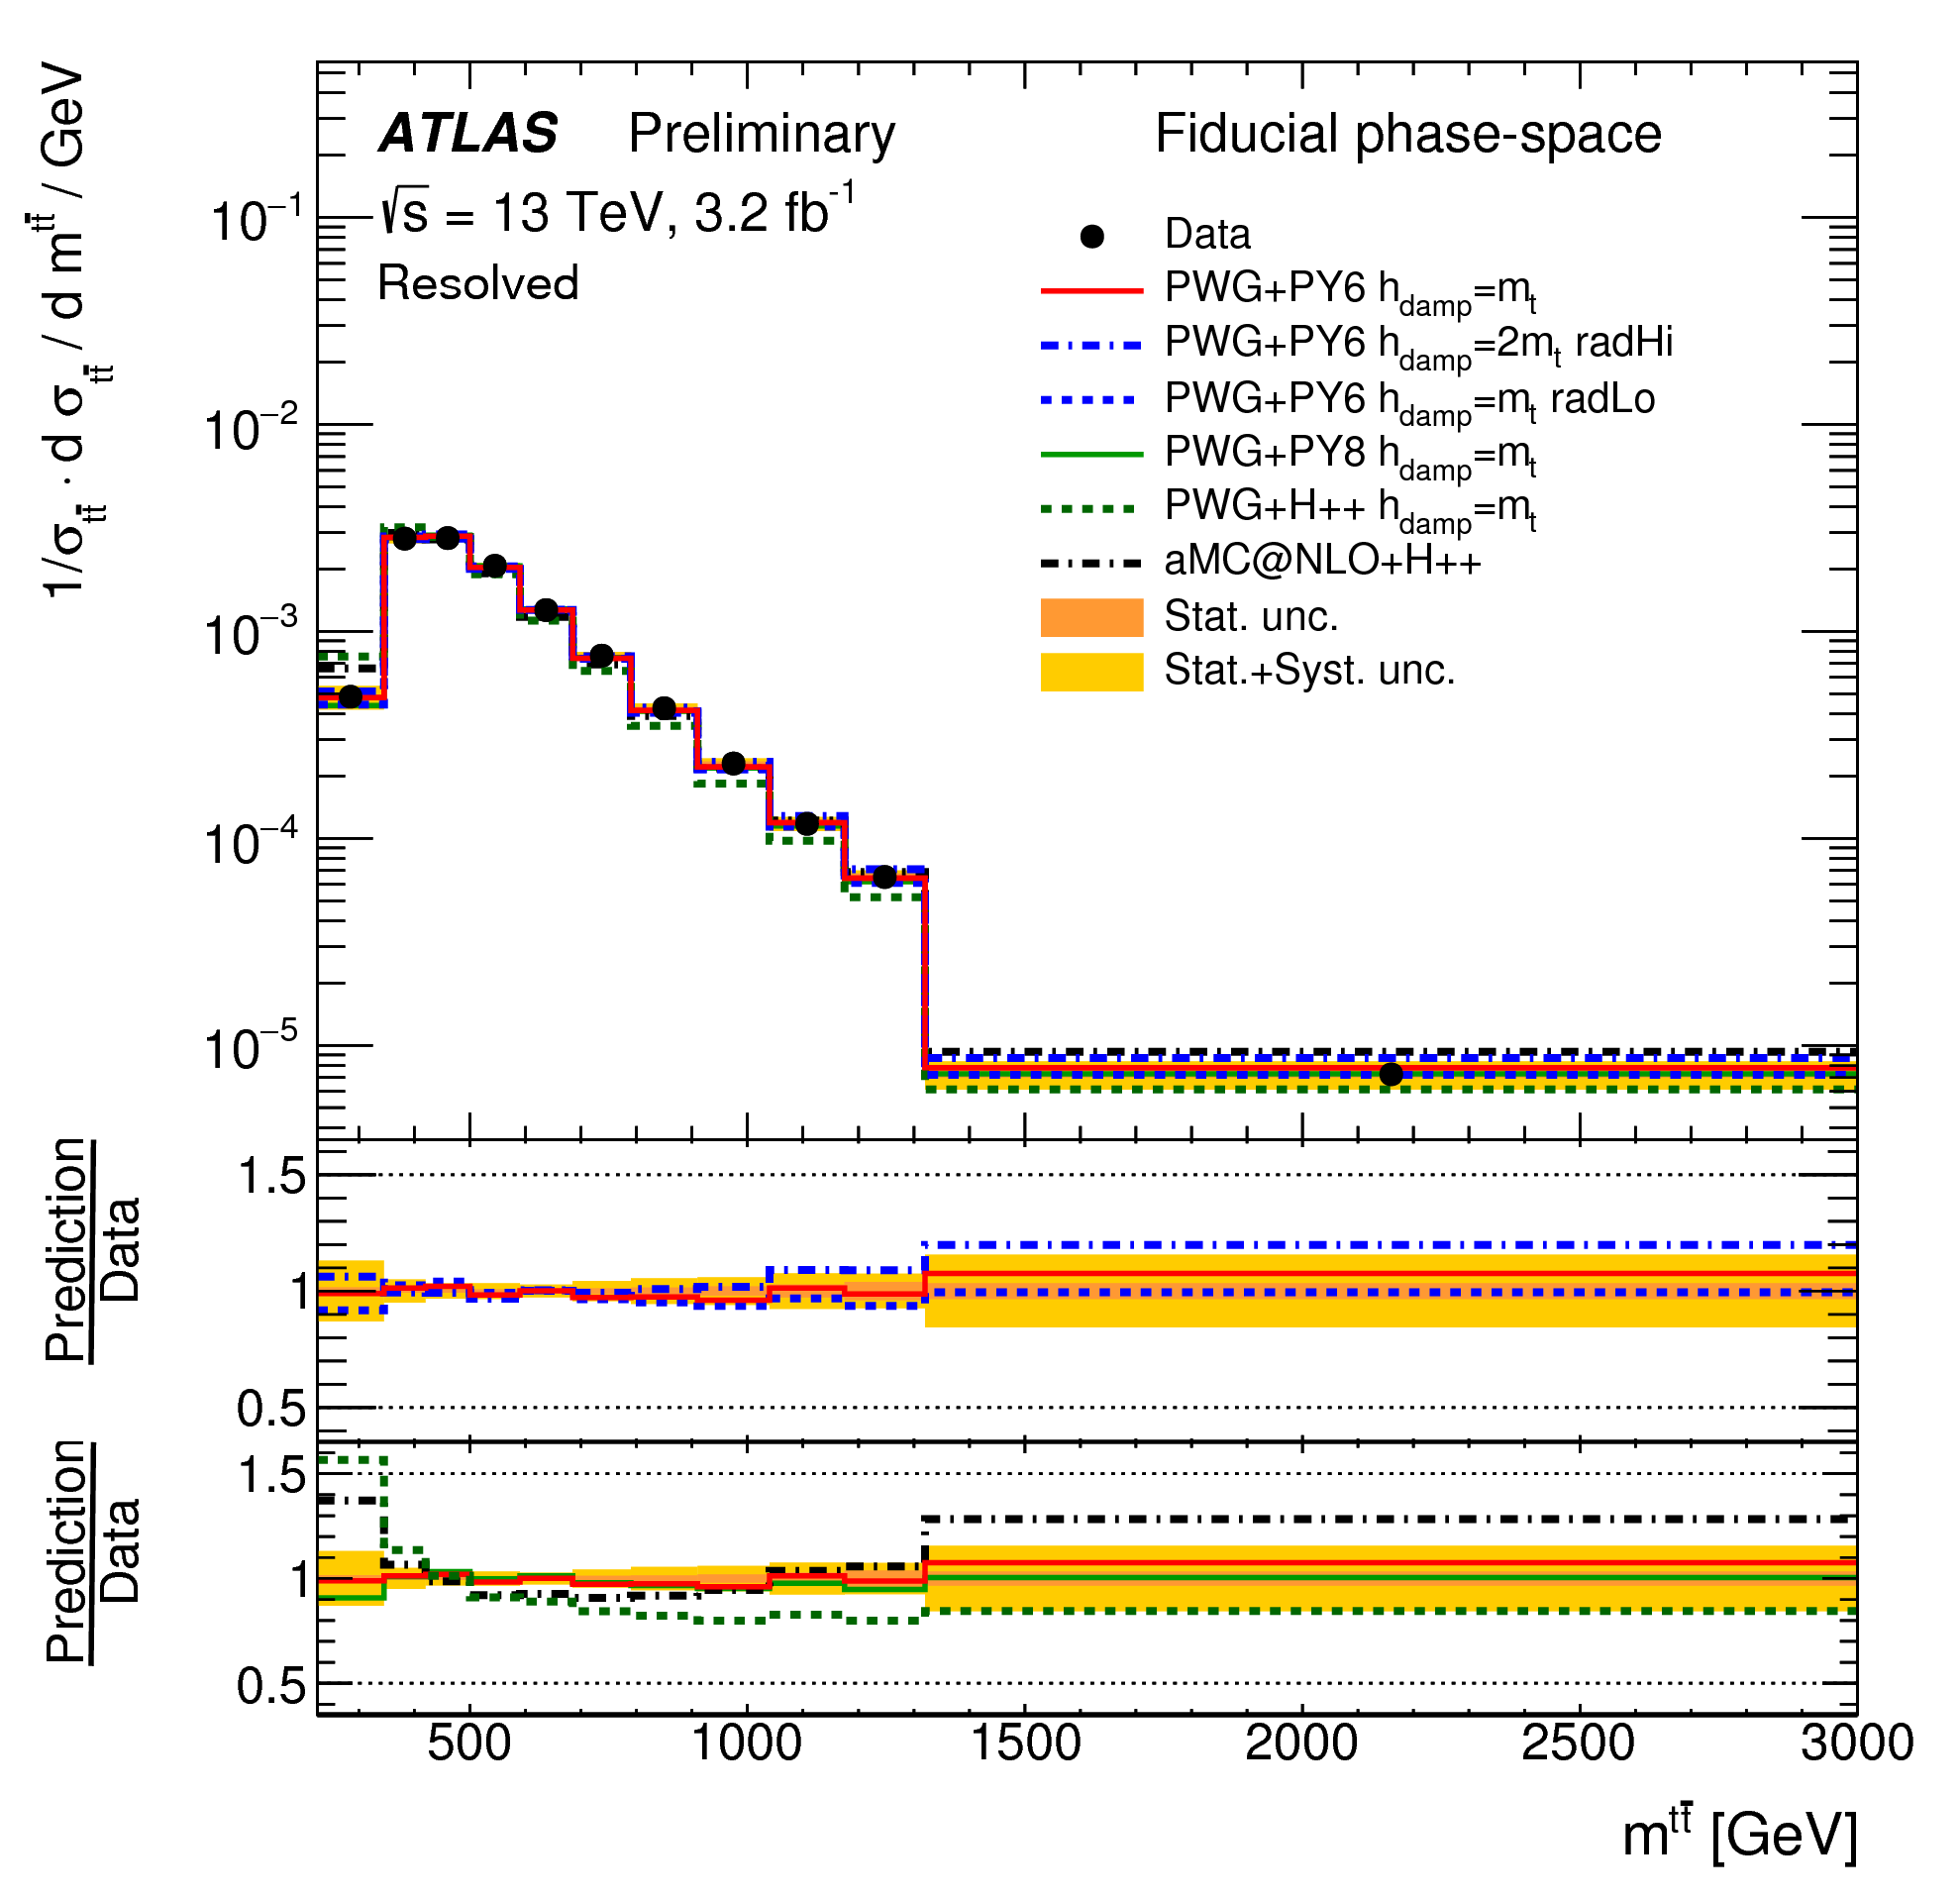
\includegraphics[width=0.70\textwidth]{./figures/strategy/ttbar_mtt.png}
	\caption[Normalized $\ttbar$ differential cross section as a function of $m^{t\tbar}$]{Normalized $\ttbar$ differential cross-section as a function of $m^{t\tbar}$.  $m^{t\tbar}$ distribution falls exponentially and the $m^{t\tbar}$ is directly related to the amount of back-to-back boost between the two tops. \cite{ttbarDiffCross} }
\label{fig:ttbar:mtt}
\end{figure}

\indent Figure \ref{fig:ttbar:3pop} illustrates example events from the two $\ttbar$ populations alongside a stop signal event for comparison.  We line up all three events according to their thrust axis and the hemisphere containing the $\MET$ is displayed in the upper half of the figure.  \\

\begin{figure}[h!]
  \centering
	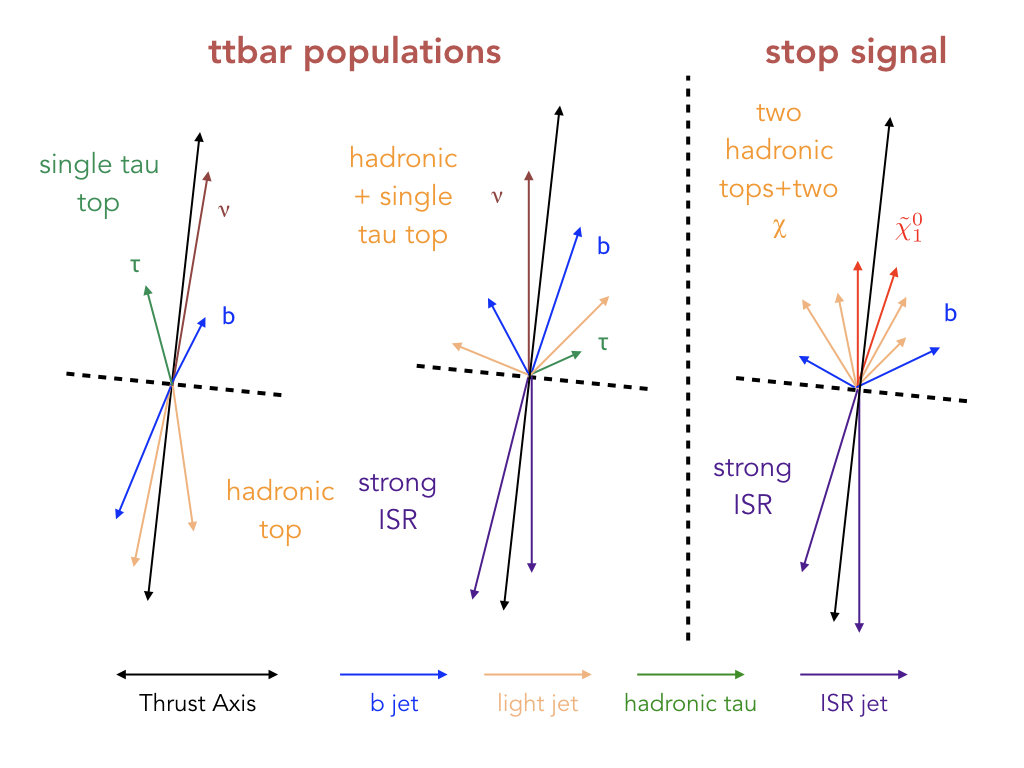
\includegraphics[width=0.85\textwidth]{./figures/strategy/ttbar_vs_signal.png}
\caption[Schematic depiction of example events from the $\ttbar$ back-to-back population, the $\ttbar$+hard ISR population, and the stop+hard ISR signal after the zero-lepton preselection]{Schematic depiction of example events from the $\ttbar$ back-to-back population, the $\ttbar$+hard ISR population, and the stop+hard ISR signal after the zero-lepton preselection.  All three events are aligned with one another according to their thrust axis.  The hemisphere containing $\met$ is located in the upper half of the figure.  The stop signal has much higher jet multiplicity and total energy in the hemisphere containing $\met$ than the $\ttbar$ back-to-back population. }
\label{fig:ttbar:3pop}
\end{figure}

\indent We can immediately see that the signal has significantly higher jet multiplicity and total energy in the hemisphere with the $\MET$ than the $\ttbar$ back-to-back population in $\ttbar$.  The signal has six jets originating from the two hadronic top decays in the hemisphere plus the $\MET$ from two neutralinos in the same hemisphere.  In comparison, the $\ttbar$ back-to-back event only has decay products from a single leptonic top in the hemisphere containing $\met$.   The $\ttbar$+hard ISR population has higher jet multiplicity and energy in the $\MET$ hemisphere. However, it still has on average less total energy and jet multiplicity than the stop signal.  \\

\indent By placing requirements on the jet multiplicity and total energy in the hemisphere with $\MET$, the signal region selections are able to reject over 99.5\% of $\ttbar$ events with less than 400 GeV of true ISR $\pt$.  The acceptance of $\ttbar$ events increases with true ISR $\pt$ but only asymptotically.  Even at 1200 GeV of true ISR $\pt$, a $\ttbar$ event which already passed zero-lepton preselection only has an 8\% chance of passing the additional signal region selection.  \\

\indent The signal region selection efficiency for $\ttbar$ as a function of ISR $\pt$ is shown in Figure \ref{fig:ttbar:SRaccept}.  \\

\begin{figure}[h!]
  \centering
	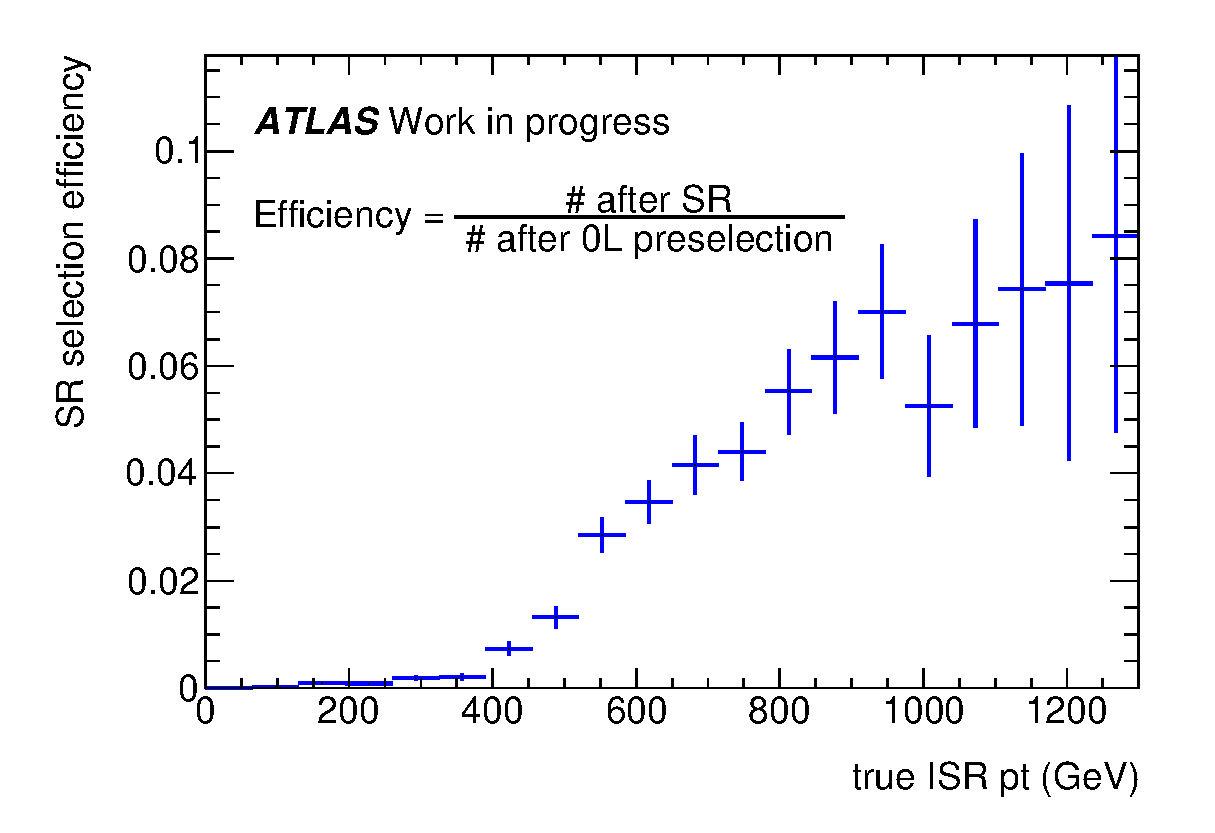
\includegraphics[width=0.85\textwidth]{./figures/strategy/Compare0L_truth_acceptance.eps}
\caption[The selection efficiency for $\ttbar$ as a function of ISR $\pt$ for $\ttbar$ after the zero-lepton preselection and after all signal region selections]{The selection efficiency for $\ttbar$ as a function of ISR $\pt$ for $\ttbar$ after the zero-lepton preselection and after all signal region selections. The selections overwhelmingly reject $\ttbar$ with low ISR $\pt$, rising to around 8\% for $\ttbar$ with 1 $\tev$ of ISR $\pt$ }}
\label{fig:ttbar:SRaccept}{
\end{figure}

\indent After signal region selections, only approximately 10\% of all $\ttbar$ events have true ISR $\pt$ less than 400 $\gev$.  A back-of-the-envelope calculation shows that $\ttbar$ events need around 600 $\gev$ of ISR $\pt$ in order to boost the neutrino past the 250 $\gev$ $\met$ selection if both tops started at rest.  Such high ISR $\pt$ is required because the neutrino must share the total $t\tbar$ $\pt$ with the 5 other particles in the $\ttbar$ decay.  This completely agrees with the true ISR $\pt$ distribution in the signal region which peaks around 550-600 $\gev$ for $\ttbar$ background.  \\

\indent The $\ttbar$ true ISR $\pt$ distribution after the zero-lepton preselection and after signal region selections can be seen in Figure \ref{fig:ttbar:SR:trueISRpt_presel_SRC}.  \\

\begin{figure}[h!]
  \centering
	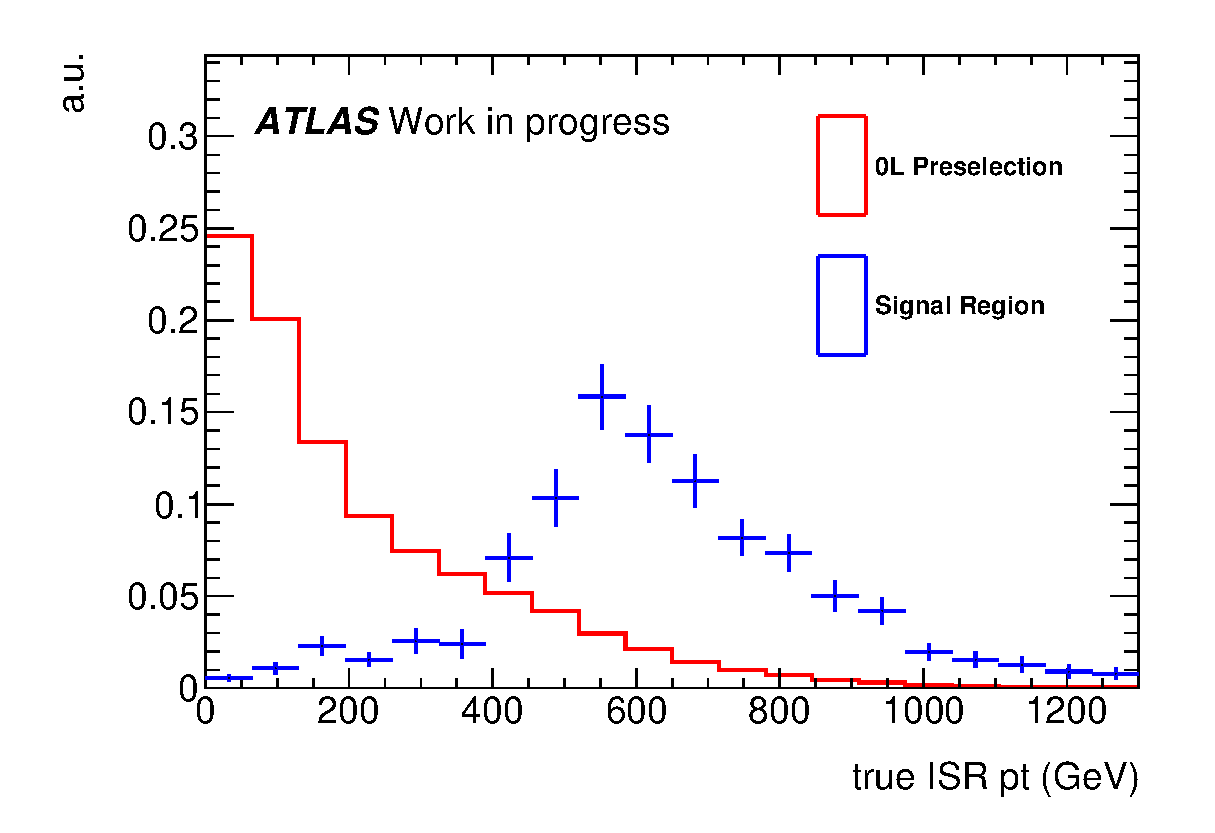
\includegraphics[width=0.85\textwidth]{./figures/strategy/Compare0L_truth.eps}
\caption[Distribution of true ISR $\pt$ for $\ttbar$ after the zero-lepton preselection and after all signal region selections]{Distribution of true ISR $\pt$ for $\ttbar$ after the zero-lepton preselection and after all signal region selections.  Both distributions have been normalized to unit area.}
\label{fig:ttbar:SR:trueISRpt_presel_SRC}
\end{figure}

\section{Order of Magnitude Estimation of how Signal Region Selections Improve Signal over Background Ratio}
\label{sec:SR:estimate}

\indent The signal region selects for $\ttbar$ with at least 550 $\gev$ of ISR $\pt$.  In comparison, the stop signal with $m_{\stop} = 400 \gev$ requires only 440 $\gev$ of ISR $\pt$ to pass the $\met > 250 \gev$ requirement and the signal region selections due to the $\met \sim m_{\ninoone}/m_{\stop} \times \PTISR $ relationship.  \\

\indent The normalized $\ttbar$ differential cross section as a function of $p_{T}^{t\tbar}$ can be seen in Figure \ref{fig:ttbar:ttpt}.  $p_T^{t\tbar}$ is equal to the true $\PTISR$ because anything that the $\ttbar$ recoils against is considered ``ISR'' by the ISR identification algorithm.  By extrapolating the $\ttbar$ differential cross section measurement to high $p_T^{t\tbar}$ we can see that there is approximately an order of magnitude increase in differential cross section if we decrease the ISR $\pt$ requirement by 150 $\gev$.  Therefore, the signal has a order of magnitude larger normalized differential cross section than the SM $\ttbar$ background because the signal requires less ISR $\pt$.   This equals an increase in the signal over background ratio (S/B) by a factor of $\sim10$. \\

\indent In addition, the stop signal has an higher probability of having high ISR $\pt$ than SM $\ttbar$.  This is because 440 $\gev$ of ISR $\pt$ is relatively small when compared to the two 400 $\gev$ stops.  In comparison, 440 $\gev$ is large relative to the mass of two top quarks at $\sim172.5 \gev$ each.  This means the gain in S/B from the lower signal ISR $\pt$ requirement is even larger than what Figure \ref{fig:ttbar:ttpt} suggests.  \\

\begin{figure}[h!]
  \centering
	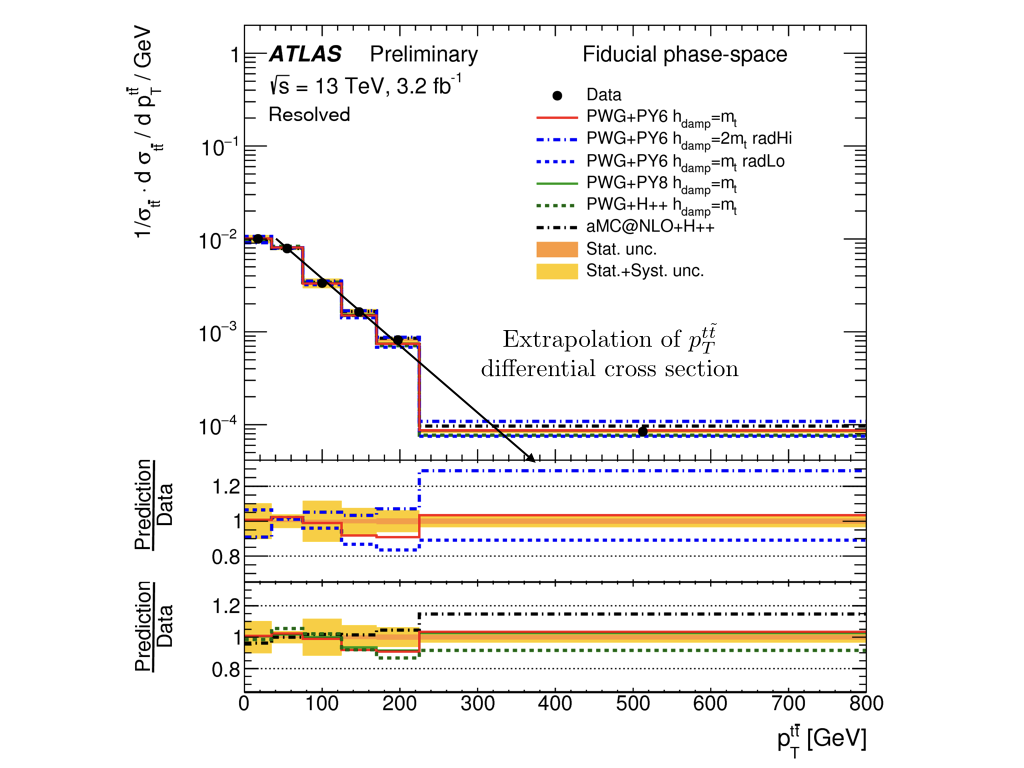
\includegraphics[width=0.70\textwidth]{./figures/strategy/ttbar_pt.png}
	\caption[Normalized $\ttbar$ differential cross section as a function of $p_T^{t\tbar}$]{Normalized $\ttbar$ differential cross-section as a function of $p_T^{t\tbar}$.\cite{ttbarDiffCross}  $p_T^{t\tbar}$ is equal to the $\PTISR$ because our ISR identification algorithm reconstructs anything that recoils against the $\ttbar$ as ISR.  $p_T^{t\tbar}$ distribution falls exponentially and can be modeled by a straight-line in the log plot.  Assuming the straight-line extrapolation holds, we would expect roughly an order of magnitude increase in differential cross section if the ISR $\pt$ required decreased by $\sim150 \gev$.  }
\label{fig:ttbar:ttpt}
\end{figure}

\indent At the same time, we gain another factor of 5 improvement in S/B simply by working in the zero-lepton channel.  In the signal region, the stops decay mainly via the all-hadronic decay channel with a 44\% branching fraction.  In comparison in the signal region, 80\% of $\ttbar$ background decay via the hadronic tau channel with a branching fraction of approximately 10\%.  The $\ttbar$ single tau decay has a branching fraction of approximately 15\% but only about 65\% of taus decay hadronically. The $\ttbar$ decay branching fraction is shown in Figure \ref{fig:ttbardecay}.\\

\indent The $\met$ and ISR correlations in both direction and magnitude further improve the S/B ratio by another factor of 5 to 10 depending on the stop mass.  The distribution of $\dPhiISRMET$ with all other signal region selections applied is shown in Figure \ref{fig:SR:dphiISRMET}. The $\RISR$ distribution after all signal selections including the $\dPhiISRMET > 3.0 $ requirement is shown in Figure \ref{fig:SR:RISR1} \\

\indent With all these effects combined, we are able to overcome the original 300 times difference in production cross section between the 400 $\gev$ stop and SM $\ttbar$.  \\

\indent As the stop mass increases, the required ISR $\pt$ in signal decreases according to $m_{\stop}/m_{\ninoone}$, further increasing the accepted signal differential cross section, even if the signal production cross section is dropping.  At the same time, the signal will peak at higher $\RISR$ ratios where background contributions are lower.  In this way, the analysis is able to maintain sensitivity across a wide range of stop masses despite rapidly dropping signal production cross section at high stop masses.  \\

\indent After zero-lepton preselection, the S/B ratio is $1$:$40$ for a stop mass of 400 GeV.  After signal region selection, the S/B ratio improves to approximately $2$:$1$ for the same mass point.  A quantitative breakdown of signal region selections and yields is given in sections \ref{sec:SR:Selections} and \ref{sec:SR:Yields}.  \\

\indent At the same time, the same kinematic selections on jet multiplicity and total energy are also difficult for subdominant backgrounds to satisfy.  In general, it is difficult for processes such as $W$+jets, $Z$+jets, single top and QCD multijets to produce such high jet multiplicity and total energy in the same half of the event as the $\MET$.   Processes such as $W$+jets and $Z$+jets normally have the $\MET$ recoiling against other energetic jets.  Therefore, energetic jets in these processes tend to lie in the hemisphere opposite the $\MET$.  After the signal region selections, the total subdominant background contribution is around 20 to 40\% depending on $\RISR$ region.  \\

%\section{Kinematic Variables Definitions}
%\label{sec:SR:Definitions}



%\indent We construct variables that measure kinematic properties of both the ISR and sparticle hemispheres.  The variables used in the signal region definition are listed below: \\

%\begin{description}
%\item [\boldmath \nBJetS:] number of b-tagged jets associated with the sparticle hemisphere.
%\item [\boldmath \nJetS:] number of jets associated with the sparticle hemisphere.
%\item [\boldmath \pTSBZero:] $\pt$ of the leading b-jet in the sparticle hemisphere.
%\item [\boldmath \pTSFour:] $pt$ of the fourth jet ordered in $\pt$ in the sparticle hemisphere.
%\item [\boldmath \dPhiISRMET:] angular separation in $\phi$ of the ISR and the $\met$ in the CM frame.
%\item [\boldmath \pTISR:] \pt\ of the ISR system, evaluated in the CM frame.
%\item [\boldmath \mS:] transverse mass between the whole sparticle system and $\met$.
%\item [\boldmath \mV/\mS:] ratio of the transverse mass of the only the visible part of the sparticle system without $\met$ and the whole sparticle system including $\met$.
%\item [\boldmath \rISR:] Ratio between invisible system ($\met$ in CM frame) and $\pTISR$
%\end{description}



\section{Signal Region Kinematic Selection}
\label{sec:SR:Selections}

\indent The signal region kinematic selections are defined in Table \ref{tab:SignalRegionC}.\\

\indent The kinematic variables used are reconstructed using the {\tt Recursive Jigsaw} method.  A detailed description of this method and variable defined can be found in section \ref{Jigsaw:ISR}.  In short, the {\tt Recursive Jigsaw} method separates the event into two hemispheres according to the thrust axis.  The thrust axis, the axis that maximizes the amount of back-to-back $\pt$ along it, approximates the axis of back-to-back recoil between the sparticle and ISR.  The hemisphere containing the $\MET$ is considered the sparticle hemisphere, and the hemisphere opposite the $\MET$ is considered the ISR hemisphere.  All jets in the sparticle hemisphere are considered to have originated from one of the stop decays.  All jets in the ISR hemisphere are considered ISR jets.  The performance of this ISR identification algorithm can be found in section \ref{Jigsaw:Performance}. \\

\indent We also construct variables that measure kinematic properties of both the ISR and sparticle hemispheres.  These include $\NjV$ and $\NbV$, the number of jets and b-tagged jets in the sparticle system.  $\MS$, $\pTjV$, and $\pTSBZero$ are all related to the total energy in the sparticle system.  $\MS$ is the total transverse mass of the sparticle system.  $\pTjV$ is the $\pt$ of the fourth highest $\pt$ jet in the sparticle system.  $\pTSBZero$ is the $\pt$ of the highest $\pt$ b-tagged jet in the sparticle system.  $\pTISR$ corresponds to the total $\pt$ of the ISR system.  Finally $\RISR = \met/\PTISR$ and $\dphiISRI$ quantify the correlation between the ISR system and $\MET$ in both magnitude and direction. \\

\begin{table}[h!]
  \begin{center}
    \def\arraystretch{1.4}%
    \begin{tabular}{c||c|c|c|c|c} \hline\hline
      {\bf Variable} & SRC-1 & SRC-2 & SRC-3 & SRC-4 & SRC-5 \\ \hline \hline
      \nBJetS & \multicolumn{5}{c}{$\ge1$} \\
      \nJetS & \multicolumn{5}{c}{$\ge5$}  \\
      \pTISR & \multicolumn{5}{c}{$>400$ GeV}   \\ 
      \pTSBZero & \multicolumn{5}{c}{$>40\gev$}  \\ 
      \pTSFour & \multicolumn{5}{c}{$>50$ GeV}   \\ 
      \mS & \multicolumn{5}{c}{$>300\gev$}  \\ \hline
      \dPhiISRMET & \multicolumn{5}{c}{$>3.00$}  \\ \hline
      \rISR &  0.30-0.40 & 0.40-0.50 & 0.50-0.60 & 0.60-0.70 & 0.70-0.80\\  \hline \hline
    \end{tabular}
  \caption{Signal region definitions, in addition to the preselection requirements presented in Table~\ref{tab:0Lcommon}. }
  \label{tab:SignalRegionC}
  \end{center}
\end{table}%

\indent The selections on $\nJetS \ge 5$ and $\nBJetS \ge 1$ ensure that the hemisphere with $\MET$ has a high amount of jet multiplicity.  These requirements are naturally satisfied in signal events because the six jets from the two stop decays are boosted by ISR toward the same direction as the two neutralinos.  However, this requirement is more difficult to satisfy for the $\ttbar$ back-to-back population since these events contain only a single leptonic or hadronic tau top in the same hemisphere as the $\MET$.  \\

\indent The $\ttbar$+hard ISR population is able to pass this selection as both the leptonic and hadronic tops are in the sparticle hemisphere.  For this reason, the main background is comprised of $\ttbar$+hard ISR events after the sparticle jet multiplicity and the $\pTISR > 400 \GeV$ requirements.  The S/B ratio is around $1$:$5$ after these selections.  \\

\indent The $\RISR$ distribution for signal and background is shown after the requirements on $\pTISR$, $\nJetS$, and $\nBJetS$ in Figure \ref{fig:SR:jetMulti}. \\

\begin{figure}[h!]
  \begin{center}
    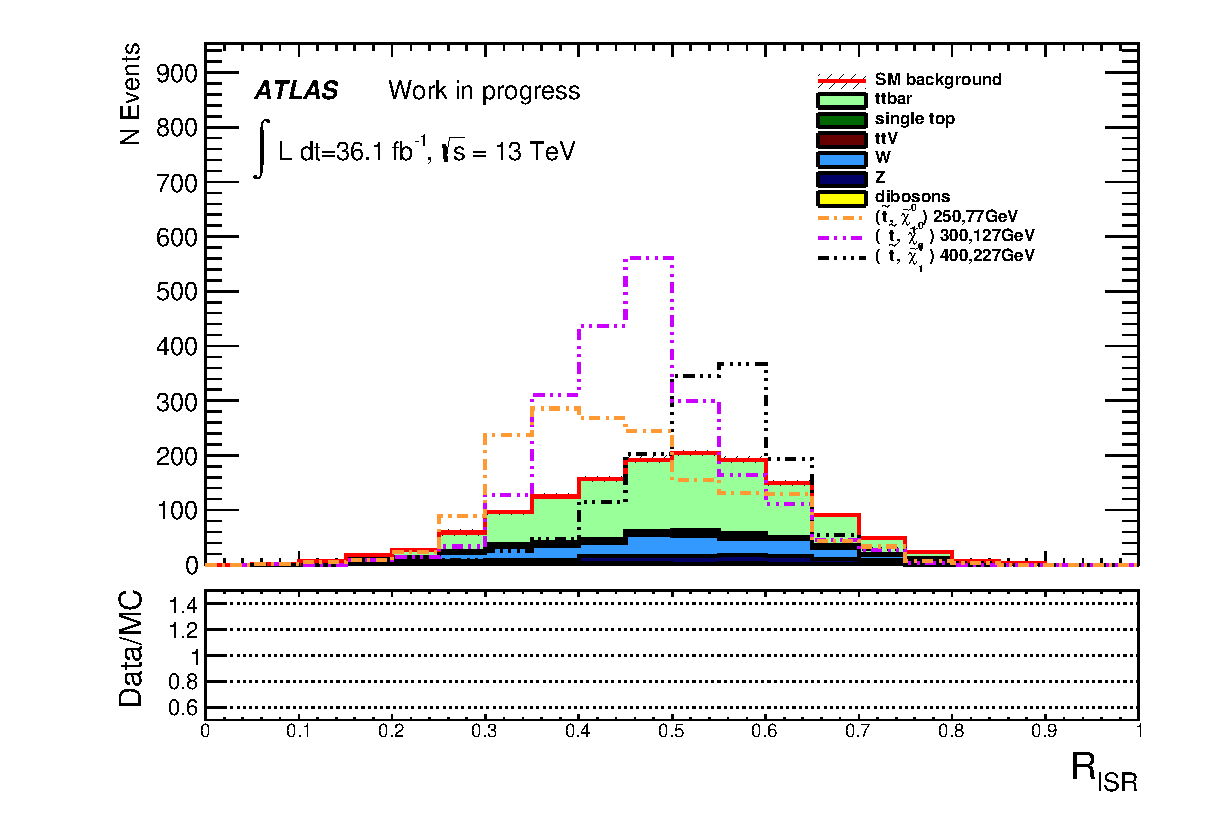
\includegraphics[width=0.80\textwidth]{figures/plotSR/SR_ND1_RISR_3SR.eps}
    \caption[$\RISR$ distribution for signal and background after preselection plus $\PTISR > 400 \gev$, $\NjV \ge 5$, and $\nBJetS \ge 1$ selections]{ $\RISR$ distribution for signal and background after preselection plus $\PTISR > 400 \gev$, $\NjV \ge 5$, and $\nBJetS \ge 1$ selections.  Stop signal rate is increased by a factor of 5 for better visibility. The hashed area in both the top and lower panel represent the uncertainty due to MC statistics.  QCD background estimation is not included.  }
  \label{fig:SR:jetMulti}
    \end{center}
\end{figure}

\indent The signal peaks in the $\RISR$ distribution after the selections on $\PTISR$, $\NjV$ and $\NbV$ (in Figure \ref{fig:SR:jetMulti}) are much sharper when compared to the $\RISR$ distribution after preselection in Figure \ref{fig:presel_dist_2}.  The high $\NjV$ and $\PTISR$ requirements select for signal events with good correlations between ISR and $\met$.  In this way, the selections on $\PTISR$, $\NjV$, and $\NbV$ increase the background rejection power of the later requirements on $\RISR$ and $\dphiISRI$.  \\

\indent The $\ttbar$ background distribution now peaks at approximately $\sim0.55$.  The $\ttbar$ events with a high $\RISR$ of $\sim0.75$ which dominated the $\ttbar$ $\RISR$ distribution after the zero-lepton preselection in Figure \ref{fig:presel_dist_2} have been rejected.  The high $\RISR$ $\ttbar$ events correspond to $\ttbar$ with hard $\ttbar$ back-to-back boost but little ISR $\pt$.  The events with lower $\RISR \sim0.5$ values correspond to $\ttbar$ with high ISR $\pt$ because $\RISR = \met/\PTISR$.  The rejection of $\ttbar$ with $\RISR \sim0.75$ is evidence that the selection is selecting mainly $\ttbar$ events with high ISR $\pt$.  \\ 

%\indent Distribution of different kinematic variables is shown after a requirement on $\pTISR$, $\nJetS$, and $\nBJetS$ is shown in figure \ref{fig:SR:jetMultiplicity}. The $\ttbar$ MC is normalized to a 1 lepton control region with the same selections on sparticle jet multiplicity, and $\pTISR$.  All subdominant background are normalized to their respective CRs defined in section \ref{sec:Bkg:sub}.\\

%\begin{figure}[htbp]
%  \begin{center}
%    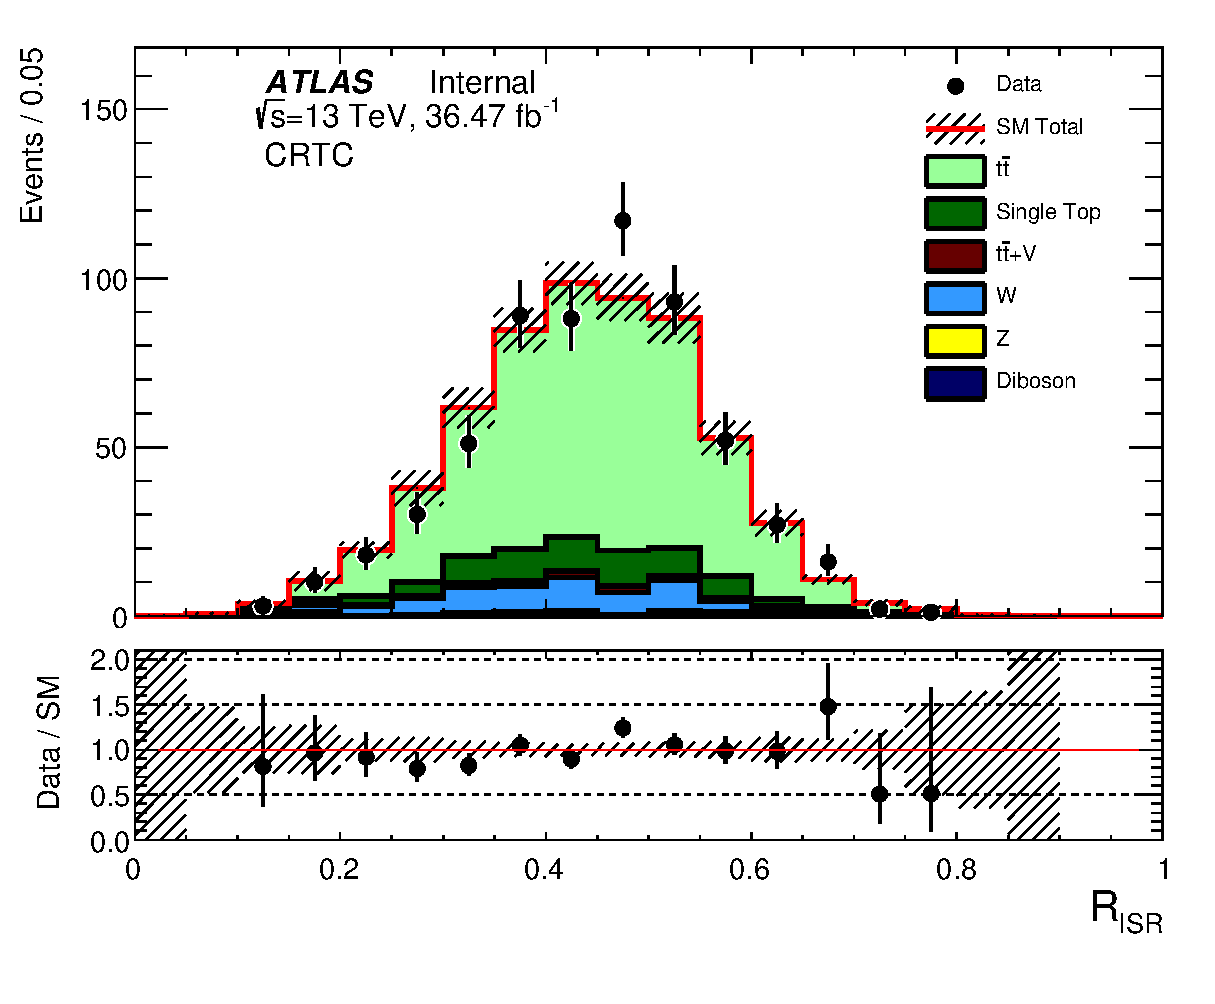
\includegraphics[width=0.45\textwidth]{figures/ttbar/postfit/CA_RISR_CRTopC}
%    \includegraphics[width=0.45\textwidth]{figures/ttbar/postfit/CA_pTISR_CRTopC}
%    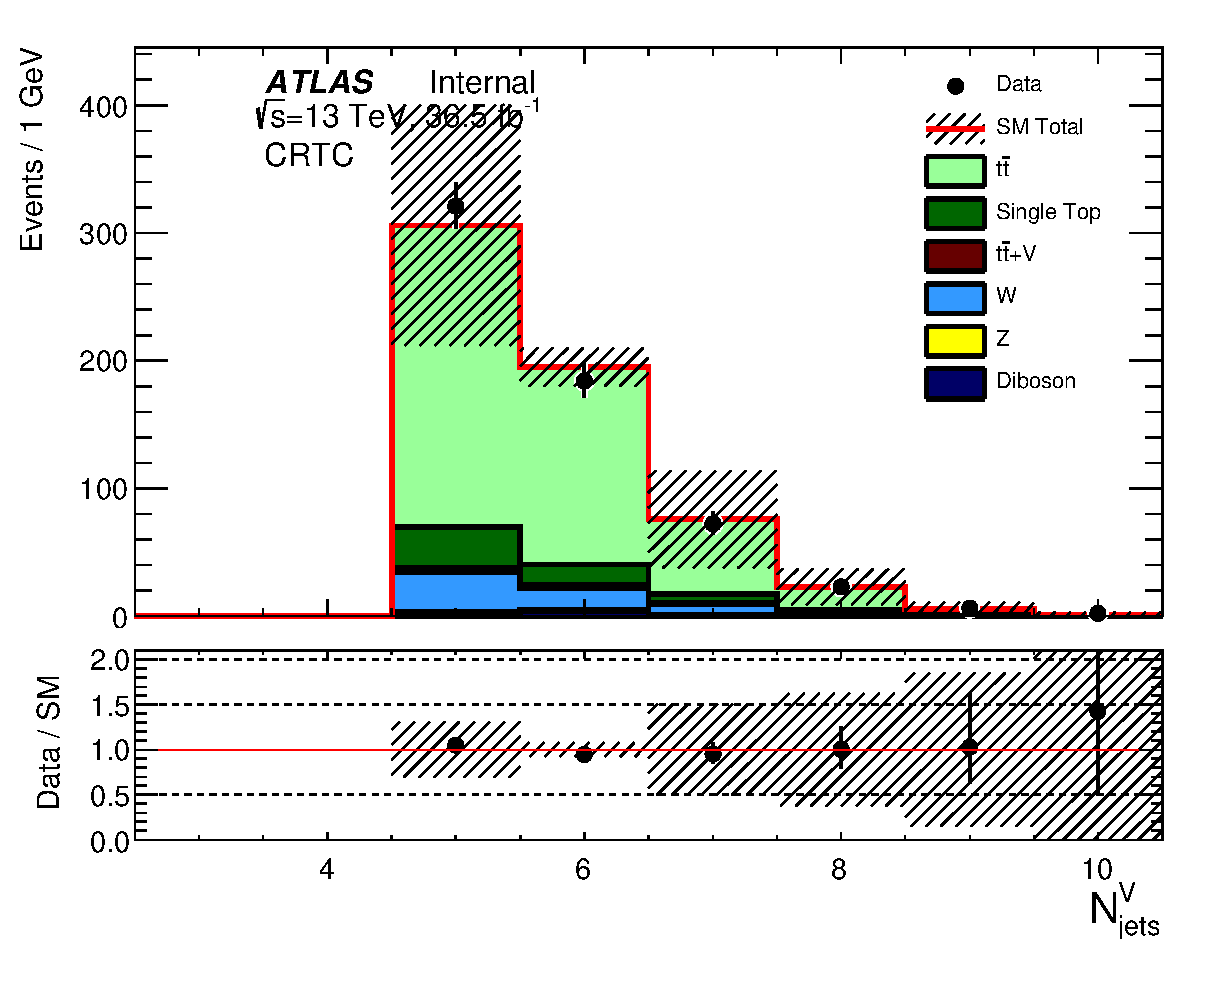
\includegraphics[width=0.45\textwidth]{figures/ttbar/postfit/CA_NjV_CRTopC}
%    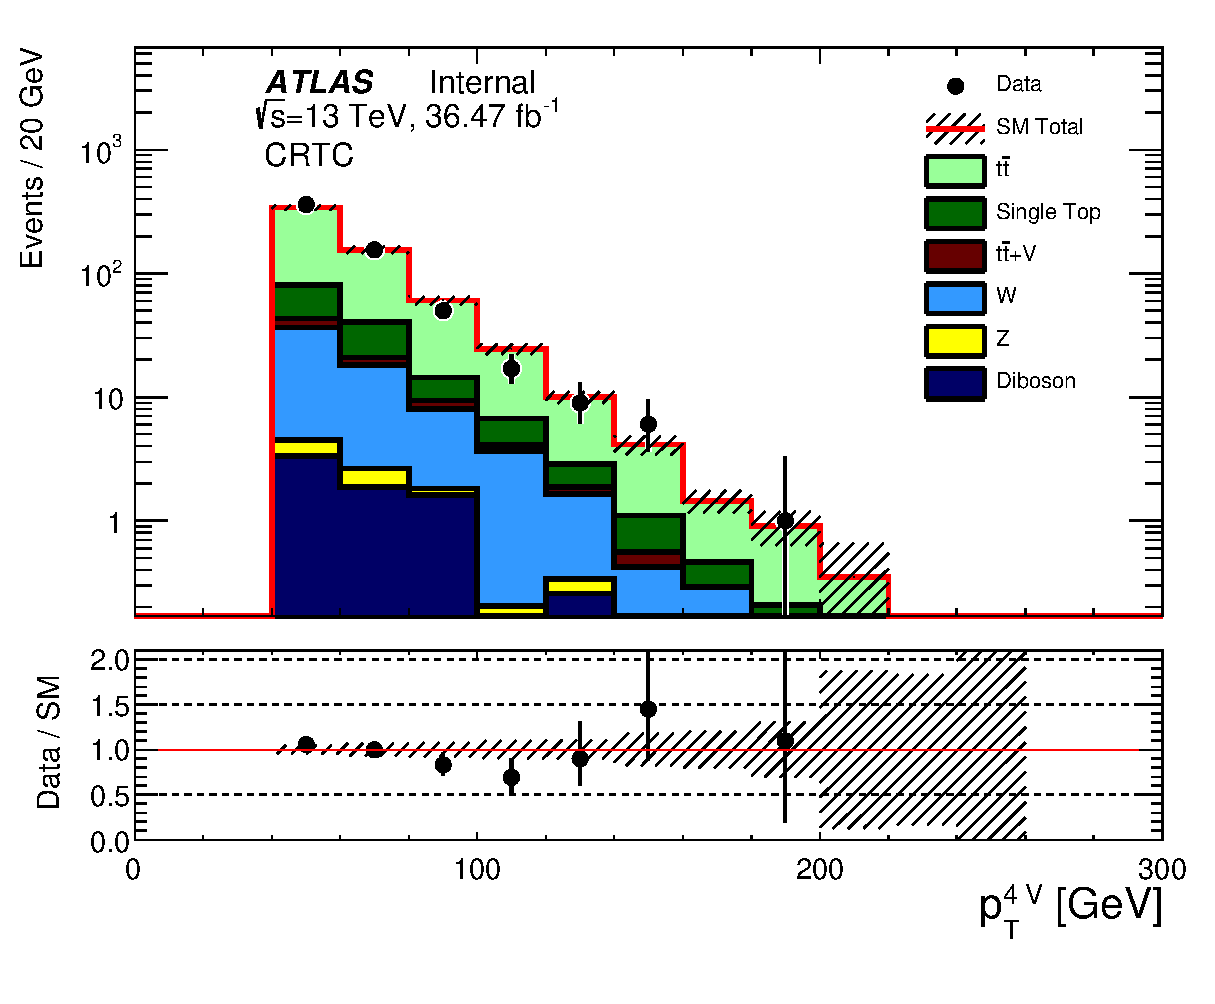
\includegraphics[width=0.45\textwidth]{figures/ttbar/postfit/CA_pTjV4_CRTopC_log}
%    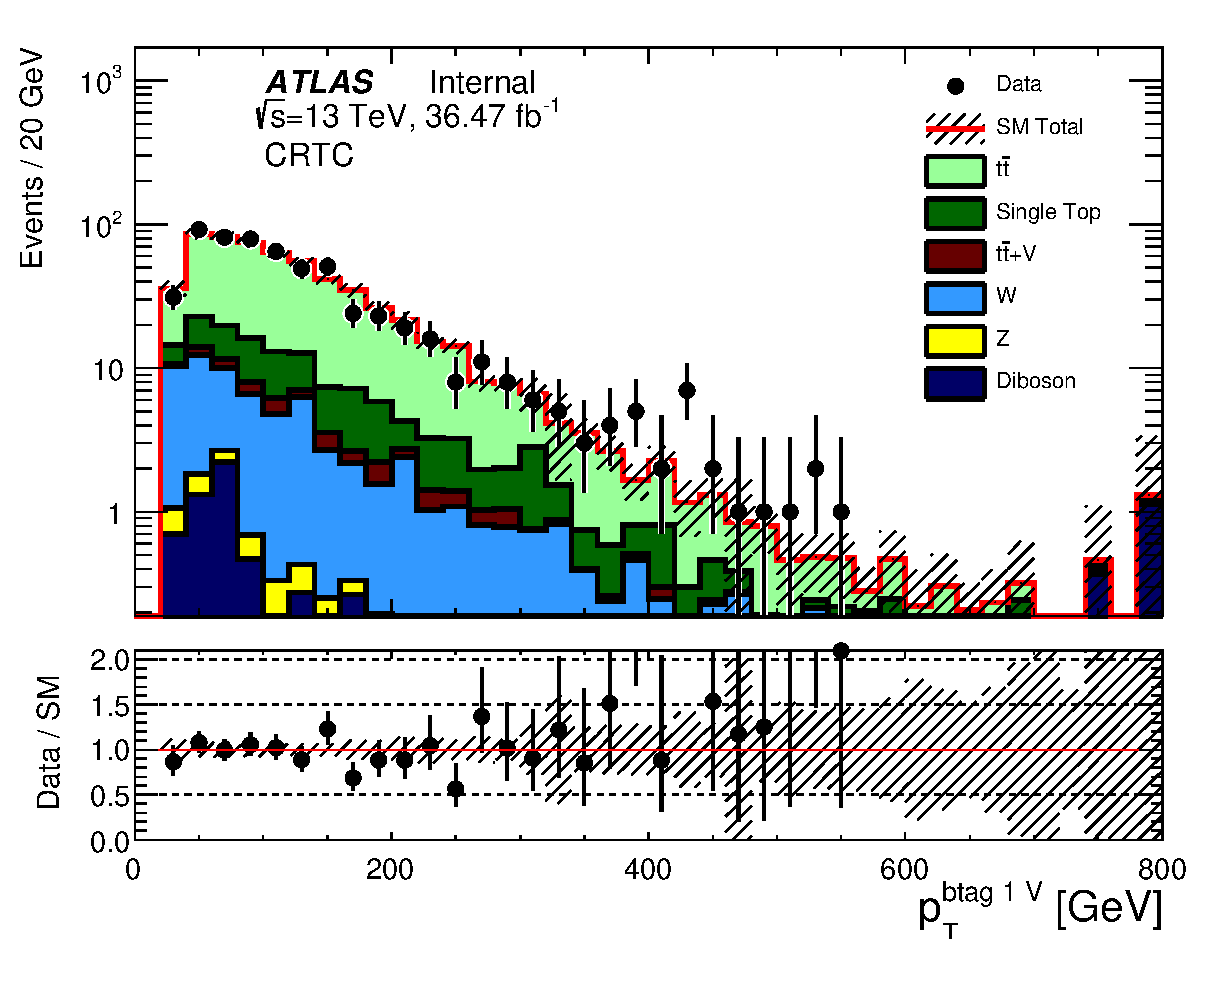
\includegraphics[width=0.45\textwidth]{figures/ttbar/postfit/CA_pTbV1_CRTopC_log}
%        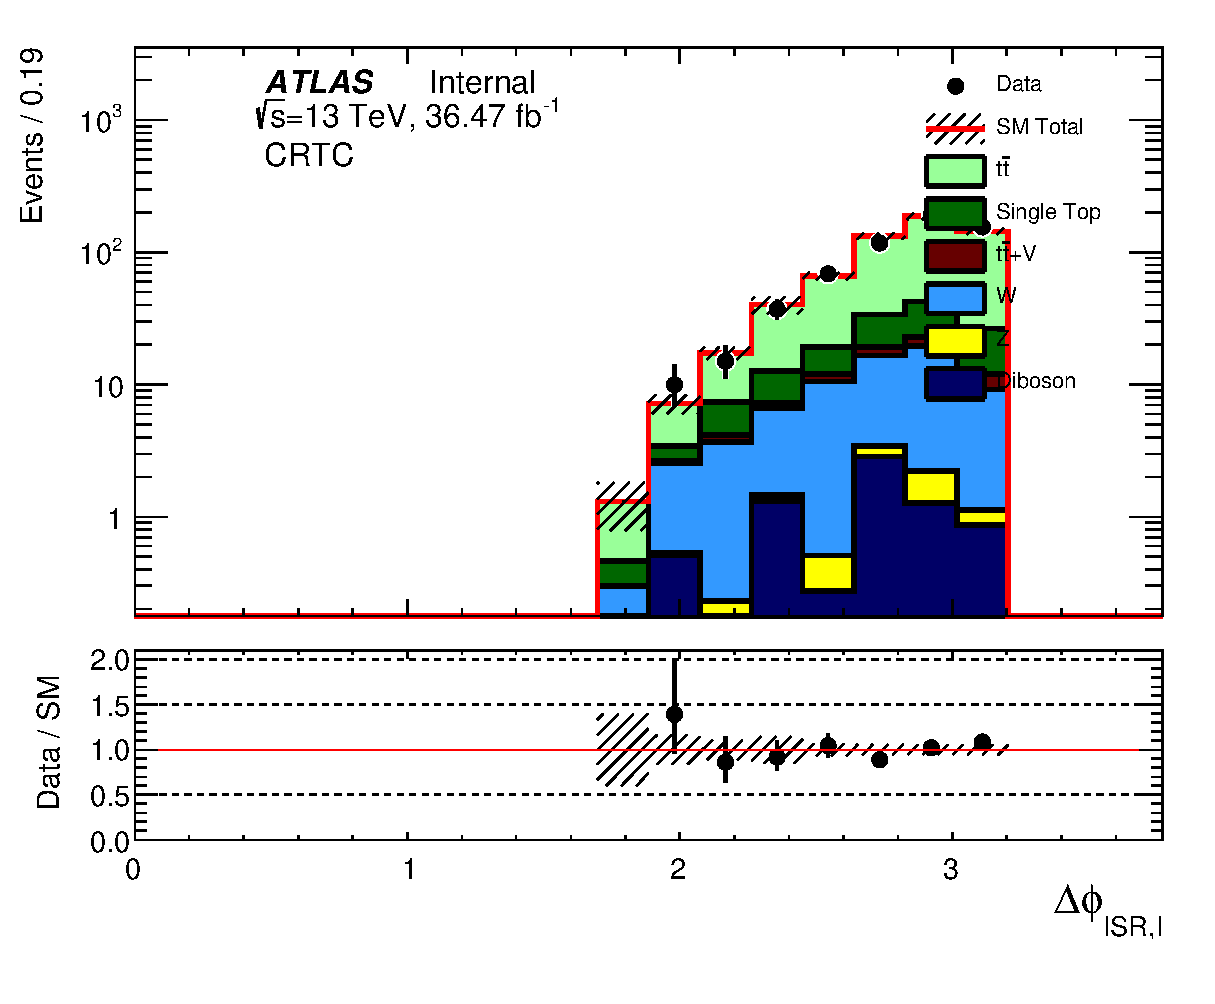
\includegraphics[width=0.45\textwidth]{figures/ttbar/postfit/CA_dphiISRI_CRTopC_log}
%  \end{center}
%  \caption{{\bf NEEDS PLOTS} Distributions for 0 lepton preselection plus $\pTISR > 400 \gev$, $\nBJetS\ge1$  and $\nJetS\ge5$ with \intlumi\ \ifb\ of data. The ratio between data and MC is shown in the bottom panel. The hashed area in both the top and lower panel represent the uncertainty due to MC statistics and detector plus theoretical systematic uncertainties}
%  \label{fig:SR:jetMultiplicity}
%\end{figure}

\indent Next, we make a requirement on the total energy of the sparticle system.  The total transverse mass of the sparticle system, $\mS$, must be greater than $300 \gev$ and $\pTSFour$, $\pt$ of the 4th highest $\pt$ jet in the sparticle system, must be greater than $50 \gev$.  $\pTSBZero$, the highest $\pt$ b-jet in the sparticle system, must also be greater than $40 \gev$.   The distributions of $\MS$, $\pTjV$ and $\pTSBZero$ after the $\NjV \ge 5$, $\NbV \ge 1$ and $\PTISR > 400 \gev$ selections are shown in Figure \ref{fig:SR:jetMulti2}. \\

\begin{figure}[h!]
  \begin{center}
    \begin{subfigure}[b]{0.40\textwidth}    
    	 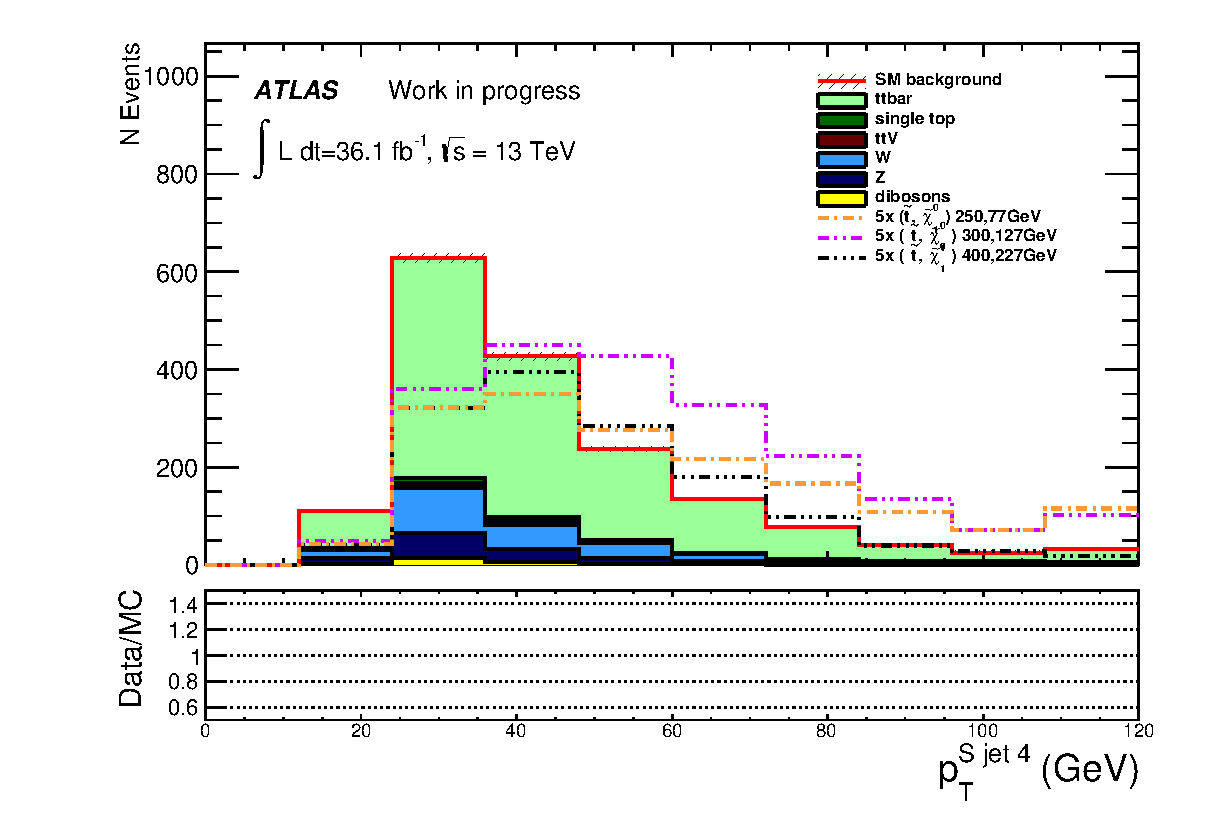
\includegraphics[width=\textwidth]{figures/plotSR/SR_ND1_pTjV4_3SR.eps}
                \caption{ }
    \end{subfigure}
    \begin{subfigure}[b]{0.40\textwidth}    
    	 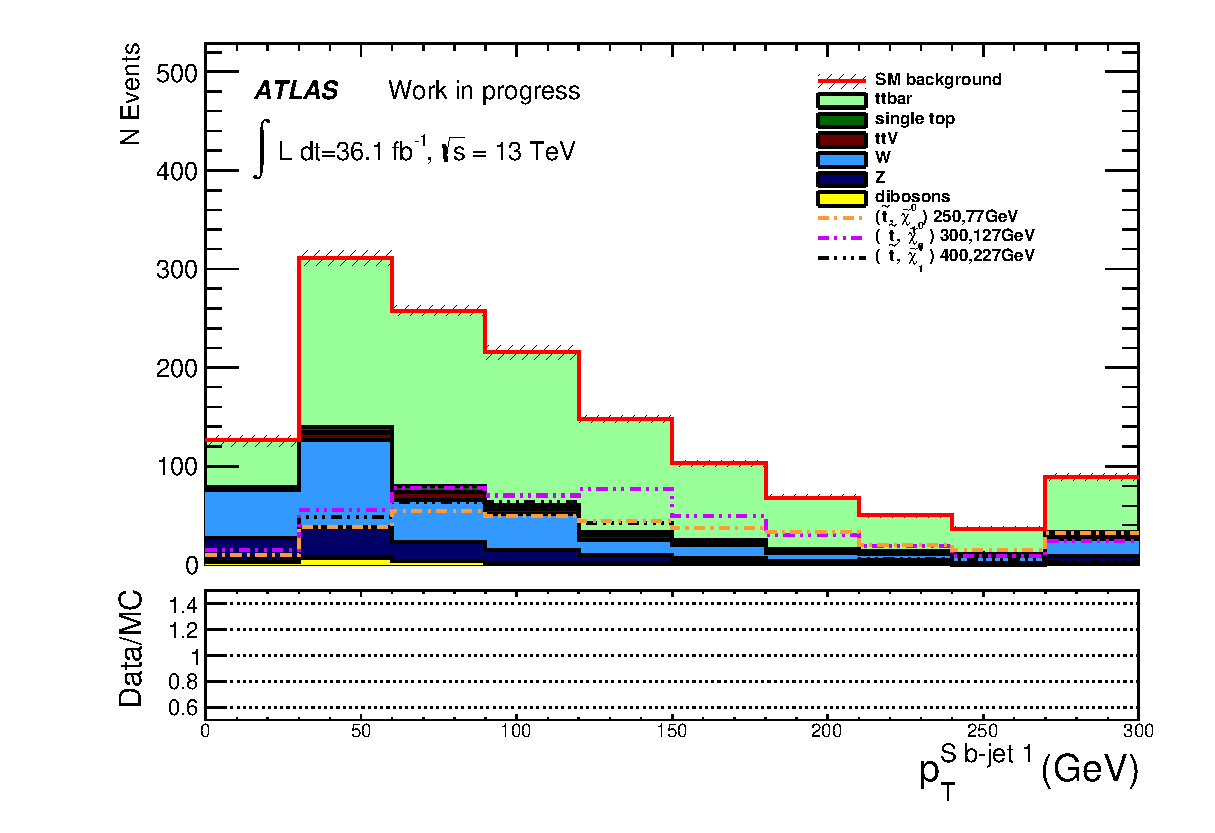
\includegraphics[width=\textwidth]{figures/plotSR/SR_ND1_pTbV1_3SR.eps}
                \caption{ }
    \end{subfigure}
    \begin{subfigure}[b]{0.40\textwidth}    
    	 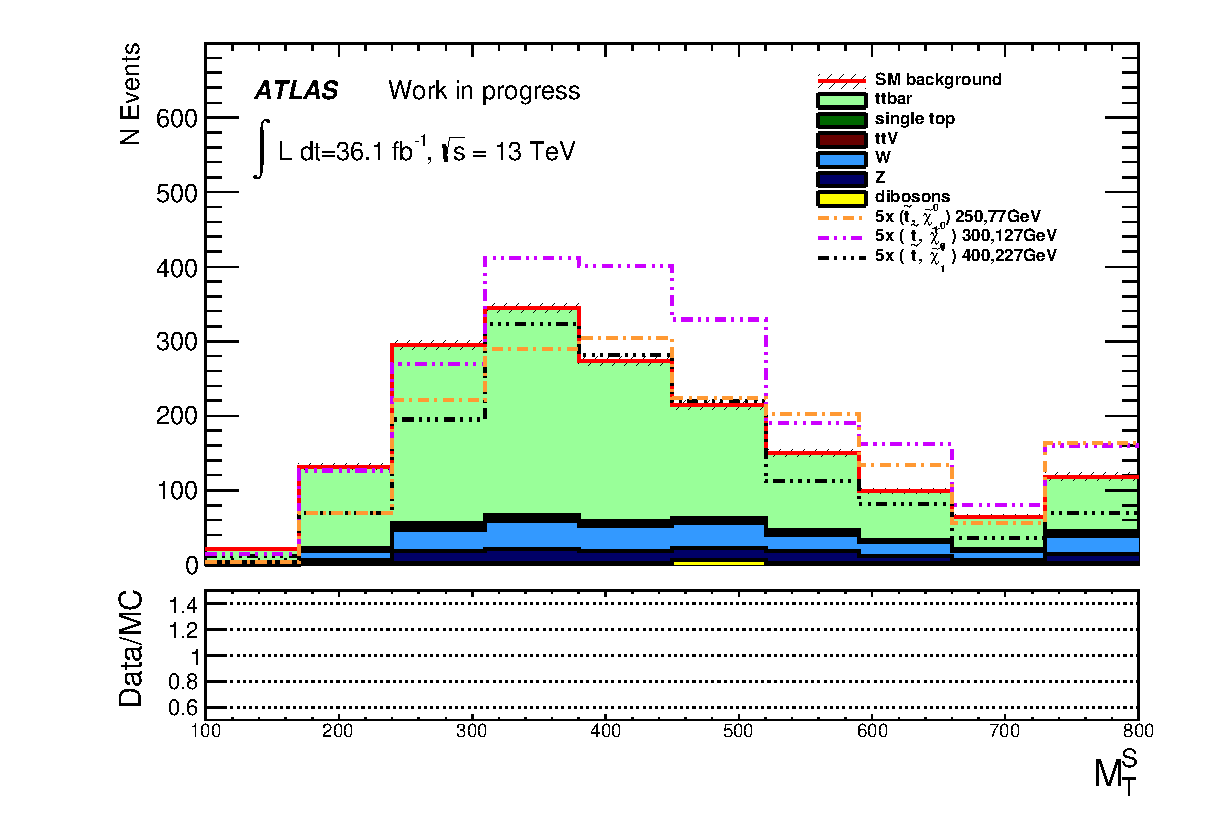
\includegraphics[width=\textwidth]{figures/plotSR/SR_ND1_MS_3SR.eps}
                \caption{ }
    \end{subfigure}
     \caption[$\MS$, $\pTjV$, and $\pTbV$ distributions for signal and background after preselection plus $\PTISR > 400 \gev$, $\NjV \ge 5$, and $\nBJetS \ge 1$ selections]{ $\MS$, $\pTjV$, and $\pTbV1$ distributions for signal and background after preselection plus $\PTISR > 400 \gev$, $\NjV \ge 5$, and $\nBJetS \ge 1$ selections.  Stop signal rate is increased by a factor of 5 for better visibility. The hashed area in both the top and lower panel represent the uncertainty due to MC statistics.  QCD background estimation is not included.  }
  \label{fig:SR:jetMulti2}
    \end{center}
\end{figure}

\indent In general, the signal with two fully hadronic tops has higher energy jets and more total energy in the sparticle hemisphere than SM $\ttbar$.  The $\ttbar$ back-to-back  population is nearly eliminated by these selections as they only have a single leptonic top in the same hemisphere as $\met$.  In $\ttbar$ events with hard ISR, the ISR boosts both tops toward the hemisphere containing $\met$.  However, the combined energy of the hadronic and leptonic tops is still less on average than the energy of two hadronic tops plus two neutralinos in the stop signal.  The $\MS > 300 \gev$, $\pTjV > 50 \gev$ and $\pTbV > 40 \gev$ requirements improve the S/B ratio to around $1$:$2$. \\

 %Of the $\ttbar$ events that passed zero-lepton preselection, less then 2\% of $\ttbar$ events with true ISR $\pt$ less then $400 \gev$ pass these additional requirements.   The $\ttbar$ that also hard ISR $\pt$ still find this requirement difficult to satisfy.  Even $\ttbar$ events with greater then $600 \gev$ of true ISR $\pt$ has a selection efficiency of approximately 35\%.  S/B ratio improves to around $1$:$2$ after these selections. \\

%\indent Distribution of various kinematic variables after sparticle jet multiplicity, $\pTISR$, and sparticle energy requirement is shown in figure \ref{fig:SR:sparticleEnergy}.  The $\ttbar$ MC is normalized to a 1 lepton control region with the same selections on sparticle jet multiplicity, $\pTISR$, and sparticle energy requirement.  All subdominant background are normalized to their respective CRs defined in section \ref{sec:Bkg:sub}.\\
%\begin{figure}[htbp]
%  \begin{center}
%    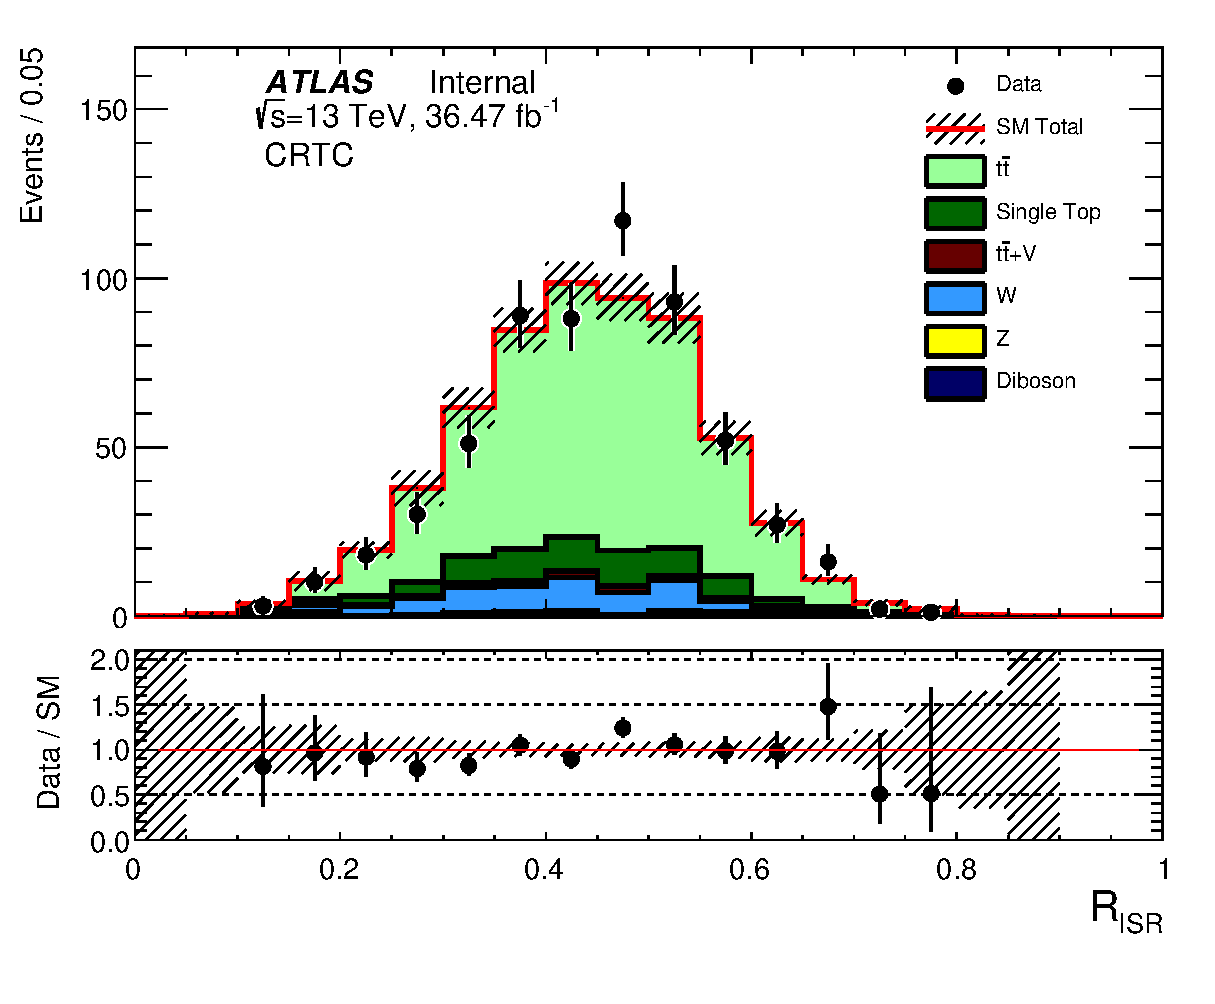
\includegraphics[width=0.45\textwidth]{figures/ttbar/postfit/CA_RISR_CRTopC}
%    \includegraphics[width=0.45\textwidth]{figures/ttbar/postfit/CA_pTISR_CRTopC}
 %   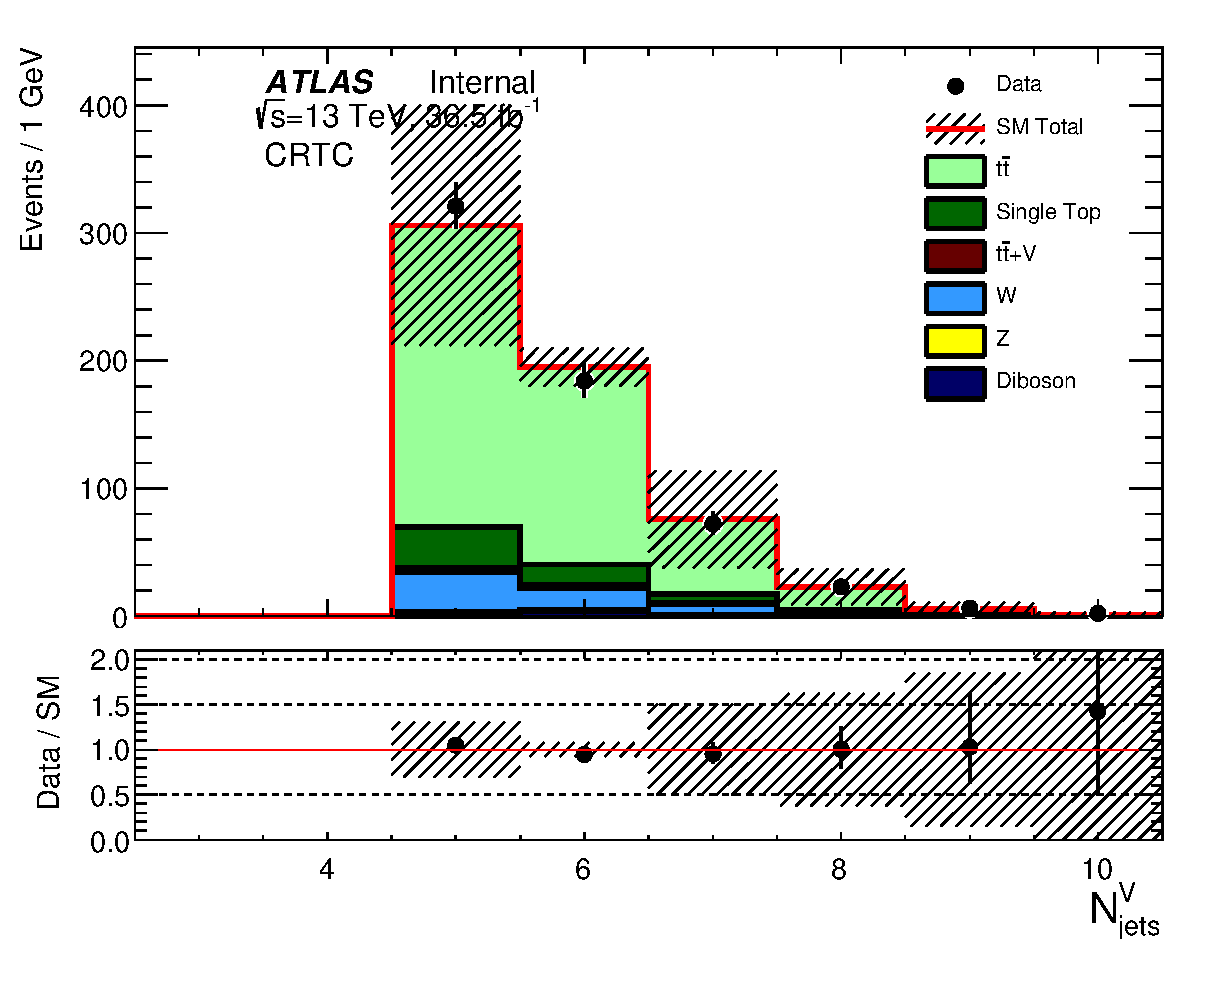
\includegraphics[width=0.45\textwidth]{figures/ttbar/postfit/CA_NjV_CRTopC}
 %   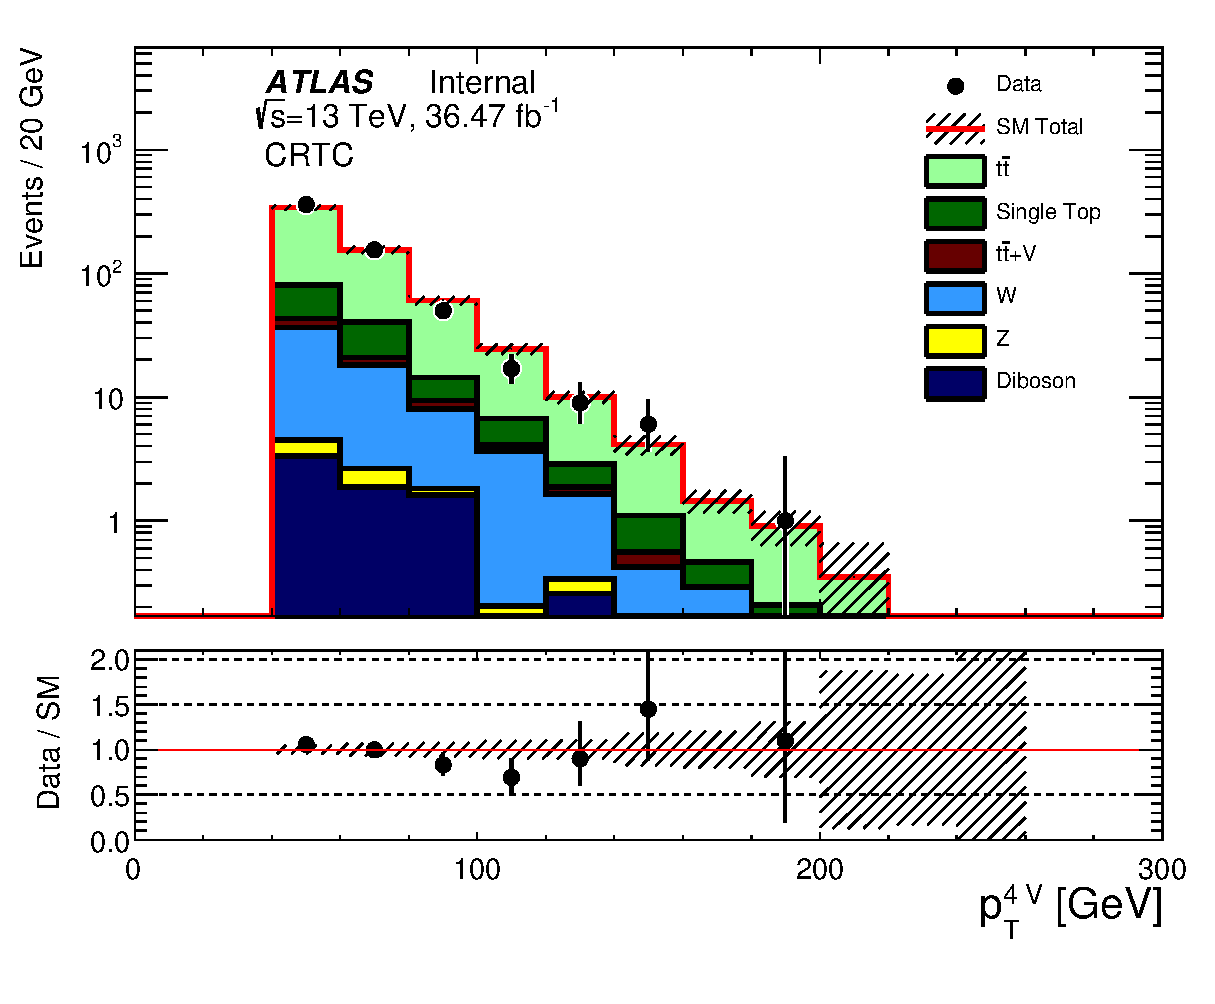
\includegraphics[width=0.45\textwidth]{figures/ttbar/postfit/CA_pTjV4_CRTopC_log}
 %   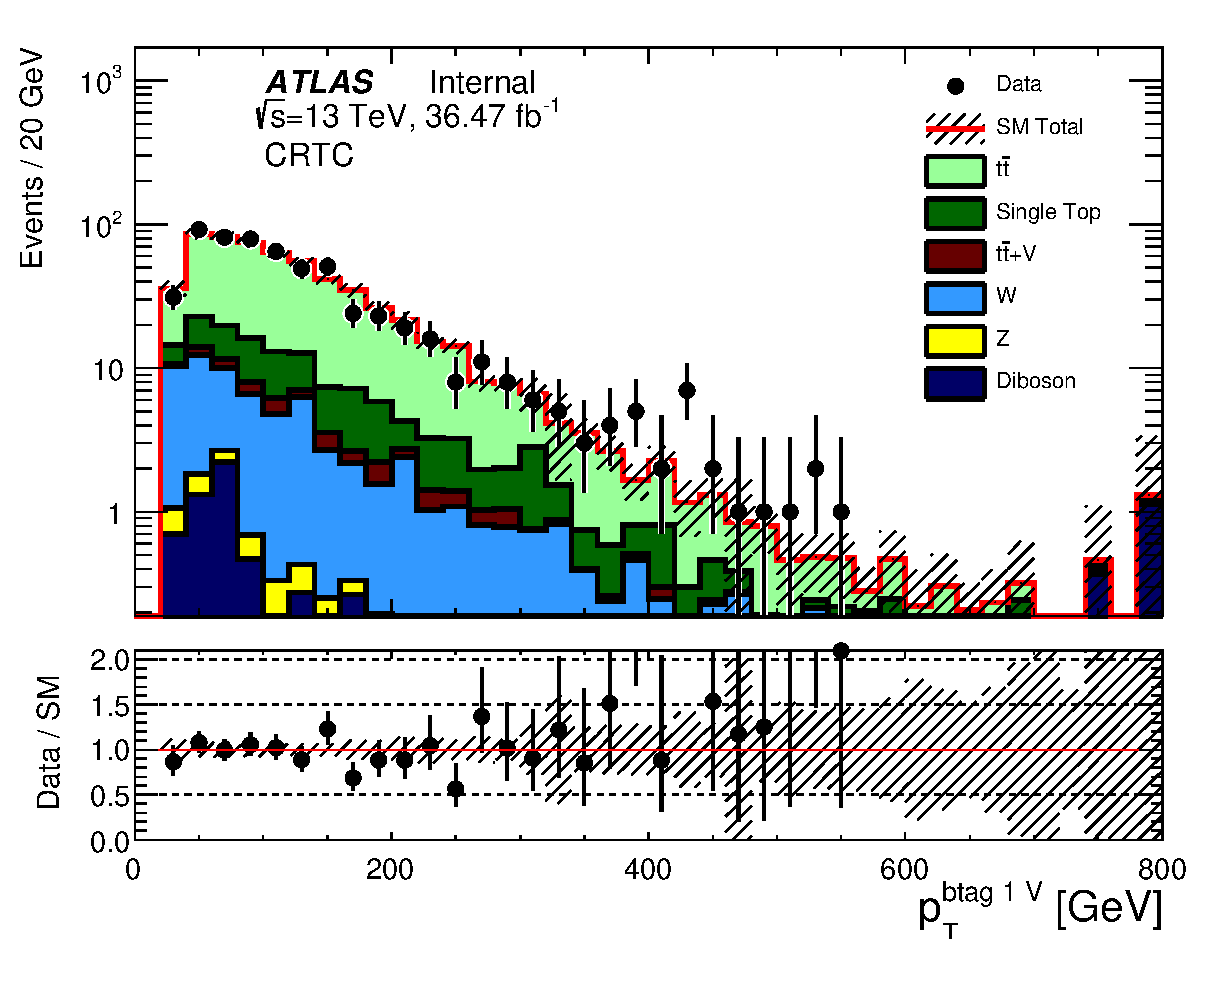
\includegraphics[width=0.45\textwidth]{figures/ttbar/postfit/CA_pTbV1_CRTopC_log}
%  \end{center}
%  \caption{{\bf NEEDS PLOTS} Distributions for 0 lepton preselection plus sparticle jet multiplicity, $\pTISR$, and sparticle total energy requirement with \intlumi\ \ifb\ of data. The ratio between data and MC is shown in the bottom panel. The hashed area in both the top and lower panel represent the uncertainty due to MC statistics and detector plus theoretical systematic uncertainties}
%  \label{fig:SR:sparticleEnergy}
%\end{figure}

\indent Lastly, we make selections based on the correlations between the $\MET$ and ISR systems.  $\dPhiISRMET > 3.0$ ensures the $\MET$ and ISR systems are back-to-back.  The ISR system and $\MET$ must be nearly back-to-back in signal because the neutralino gains momentum mainly from ISR.  On the other hand, the neutrino in SM $\ttbar$ gains significant momentum from the top decay and its correlation with ISR is not as strong. This is also true for subdominant backgrounds including $W$+jet and single top. \\

\indent The distribution of $\dPhiISRMET$ with all previous selections on $\PTISR > 400 \gev$, sparticle hemisphere jet multiplicity, and sparticle hemisphere energy is shown in Figure \ref{fig:SR:dphiISRMET}. \\  %The $\ttbar$ MC is normalized to a 1 lepton control region with the same selections on sparticle jet multiplicity, $\pTISR$, and sparticle energy requirement.  All subdominant background are normalized to their respective CRs defined in section \ref{sec:Bkg:sub}. \\

\begin{figure}[h!]
  \begin{center}
     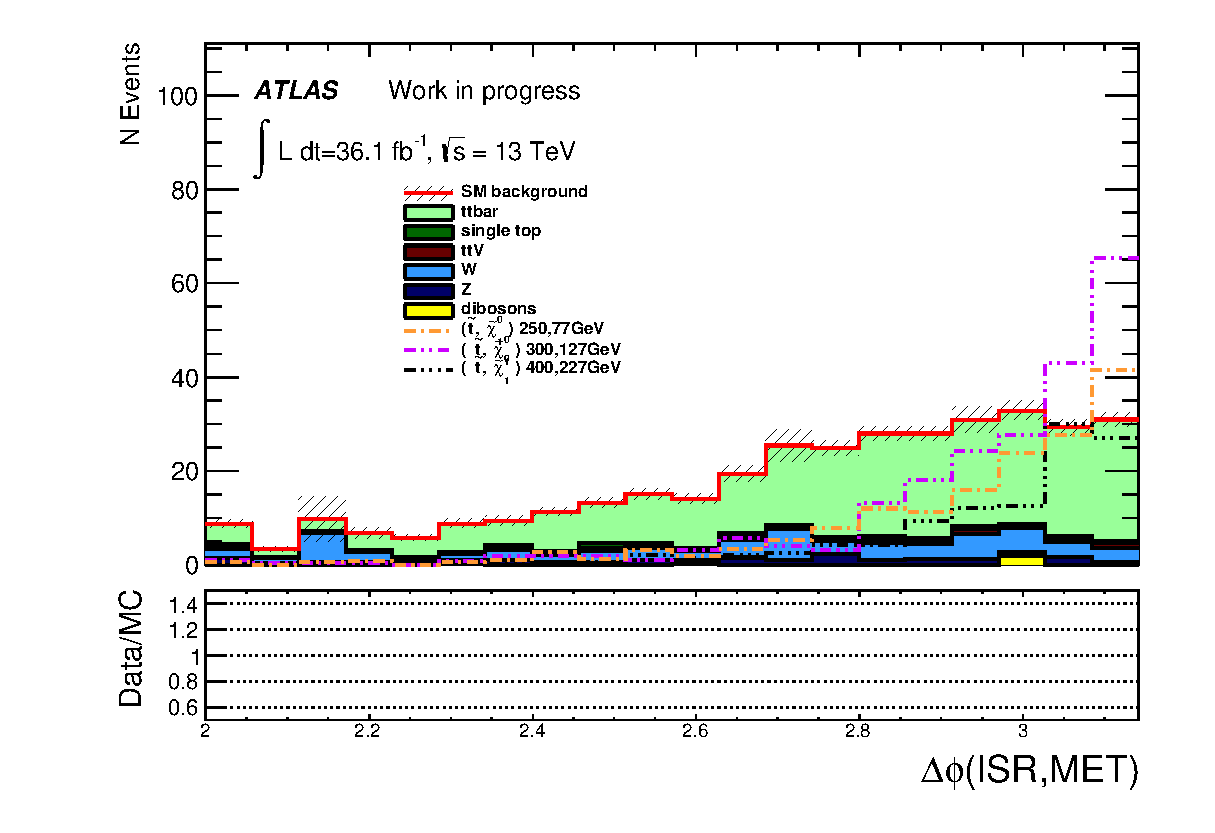
\includegraphics[width=0.80\textwidth]{figures/plotSR/SR_ND1_dphiISRI_6SR.eps}
  \caption[$\dPhiISRMET$ distribution after the zero-lepton preselection, $\pTISR > 400$ $\gev$, sparticle hemisphere jet multiplicity and sparticle hemisphere energy requirements]{$\dPhiISRMET$ distribution after the zero-lepton preselection, $\pTISR > 400$ $\gev$, sparticle hemisphere jet multiplicity and sparticle hemisphere energy requirements. The solid stacked histogram represents the expected SM background rates. The dashed histogram represent the expected number of signal events for several stop and neutralino masses. The hashed area in both the top and lower panel represents the uncertainty due to MC statistics.}
  \label{fig:SR:dphiISRMET}
    \end{center}
\end{figure}

\indent The final $\RISR$ distribution after all signal selections is shown in Figure \ref{fig:SR:RISR1}.  This $\RISR$ distribution is then separated into $5$ bins from $0.3$ to $0.8$.  The 5 signal region bins are fitted simultaneously to extract the signal strength.  We expect very few signal events in the $\RISR$ region below 0.3. The same region is also dominated by QCD background.  As such, the $\RISR$ region below 0.3 is not included in the final signal region fit.  \\

\begin{figure}[h!]
  \begin{center}
     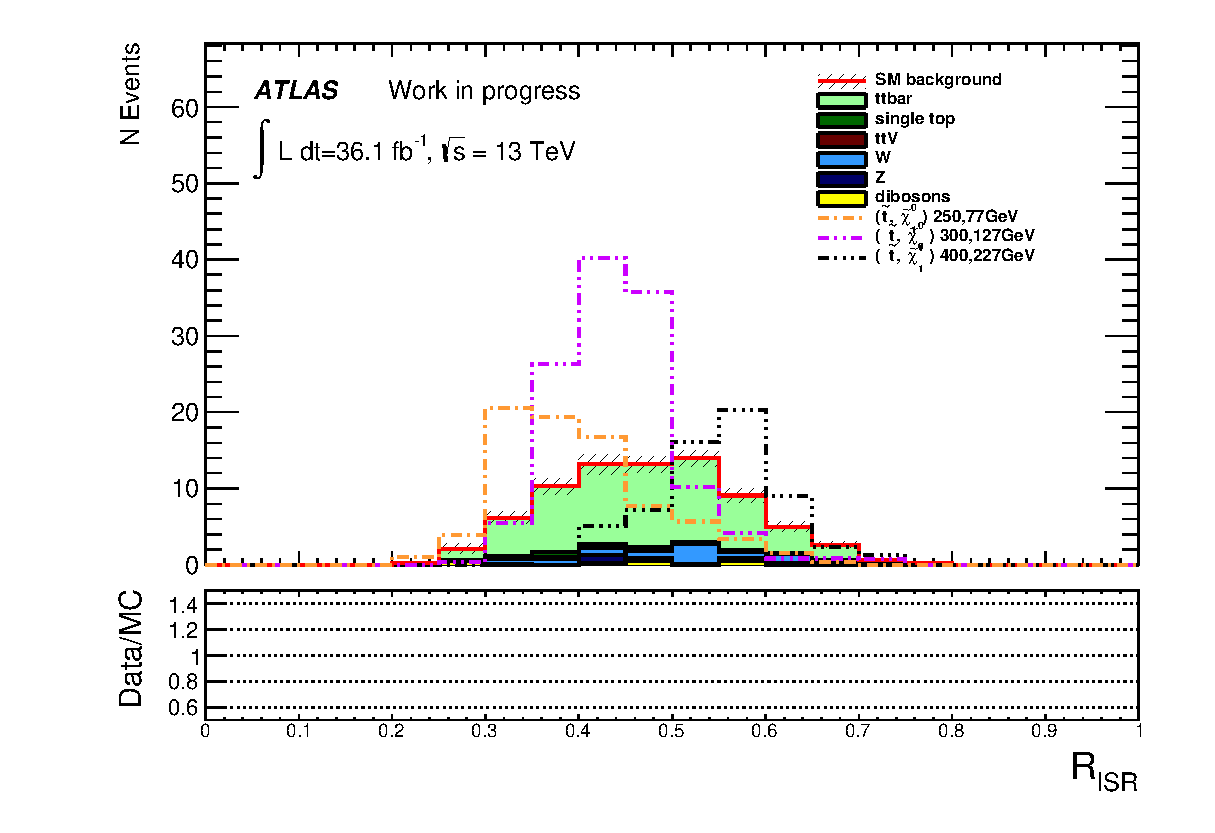
\includegraphics[width=0.80\textwidth]{figures/plotSR/SR_ND1_RISR_7SR.eps}
  \caption[$\RISR$ distribution after signal region selection corresponding to \intlumi\ \ifb\ of data]{ $\RISR$ distribution after signal region selection corresponding to \intlumi\ \ifb\ of data. The solid stacked histogram represents the expected SM background rates. The dashed histogram represent the expected number of signal events for several stop and neutralino masses. The hashed area in both the top and lower panel represents the uncertainty due to MC statistics.}
  \label{fig:SR:RISR1}
  \end{center}
\end{figure}

\indent Stop samples with different stop and neutralino masses will peak in different locations in $\RISR$ with a S/B ratio of approximately $2$:$1$ under the peak.  The simultaneous fit to all 5 bins captures this peaking feature in $\RISR$ for any stop mass.  \\

\section{Signal Region Expected Yields and Kinematic Distributions}
\label{sec:SR:Yields}

\indent The expected yields in the signal region are given in Table \ref{table.SRYields}.  Signal yields for three example signal samples with stop, neutralino masses of $(300,127 \gev), (400,227\gev), $ and $(500,327 \gev)$ are also shown for comparison.  We achieve a $1$:$1$ to $2$:$1$ S/B ratio under the signal $\RISR$ peak in the signal region. \\

\indent All expected background rates in the signal region are normalized to control regions defined in chapter \ref{chap:backgrounds}.  The control regions are designed to mimic the background kinematics in the signal region but are orthogonal to the signal region and have low expected signal rate.  We directly measure the background rate using data in the control regions and use simulation to extrapolate background predictions from the control region to the signal region. \\



\begin{table}
\begin{center}
\setlength{\tabcolsep}{0.0pc}
{\small
%%
\begin{tabular*}{\textwidth}{@{\extracolsep{\fill}}lrrr}
\noalign{\smallskip}\hline\noalign{\smallskip}
{\bf SRC yields}           & SRC1            & SRC2            & SRC3              \\[-0.05cm]
\noalign{\smallskip}\hline\noalign{\smallskip}
%%
Expected bkg events         & $21.02 \pm 6.62$          & $28.42 \pm 4.89$          & $19.60 \pm 3.53$              \\
\noalign{\smallskip}\hline\noalign{\smallskip}
%%
        Expected TTbar events         & $12.85 \pm 5.87$          & $22.05 \pm 4.19$          & $14.57 \pm 3.23$              \\
%%
        Expected Wjets events         & $0.81 \pm 0.37$          & $1.93 \pm 0.48$          & $1.91 \pm 0.63$              \\
%%
        Expected Zjets events         & 0.46 $\pm$ 0.09          & 0.90 $\pm$ 0.13          &  0.74 $\pm$ 0.15               \\
%%
        Expected TtbarV events         & $0.29 \pm 0.18$          & $0.59 \pm 0.38$          & $0.56 \pm 0.31$              \\
%%
        Expected SingleTop events         & $1.67_{-1.67}^{+2.02}$          & $1.18_{-1.18}^{+1.81}$          & $1.22_{-1.22}^{+1.37}$              \\
%%
        Expected Diboson events         & $0.39 \pm 0.33$          & $0.21 \pm 0.11$          & $0.29 \pm 0.18$              \\
%%
        Expected Multijets events         & $4.56 \pm 2.38$          & $1.58 \pm 0.77$          & $0.32 \pm 0.17$              \\
%%     
 \noalign{\smallskip}\hline\noalign{\smallskip}
$(\mstop = 300, \mLSP = 127)$ GeV & 30.68 $\pm$ 4.17 & 72.20 $\pm$ 7.29 & 14.80 $\pm$ 2.56 \\
$(\mstop = 400, \mLSP = 227)$ GeV & 1.57 $\pm$ 0.45  & 10.81 $\pm$ 1.00 & 30.01 $\pm$ 1.67 \\
$(\mstop = 500, \mLSP = 327)$ GeV & 0.11 $\pm$ 0.06  & 1.42 $\pm$ 0.26  & 6.90 $\pm$ 0.56 \\
 \noalign{\smallskip}\hline\noalign{\smallskip}

\end{tabular*}
%%%
\begin{tabular*}{\textwidth}{@{\extracolsep{\fill}}lrr}
\noalign{\smallskip}\hline\noalign{\smallskip}
{\bf SRC yields}           & SRC4            & SRC5              \\[-0.05cm]
\noalign{\smallskip}\hline\noalign{\smallskip}
%%
Expected bkg events         & $8.14 \pm 1.39$          & $0.99 \pm 0.71$              \\
\noalign{\smallskip}\hline\noalign{\smallskip}
%%
        Expected TTbar events         & $4.92 \pm 0.98$          & $0.63_{-0.63}^{+0.69}$              \\
%%
        Expected Wjets events         & $1.93 \pm 0.45$          & $0.21 \pm 0.12$              \\
%%
        Expected Zjets events         & 0.45 $\pm$ 0.24          & 0.09 $\pm$ 0.04             \\
%%
        Expected TtbarV events         & $0.08 \pm 0.08$          & $0.06 \pm 0.03$              \\
%%
        Expected SingleTop events         & $0.72_{-0.72}^{+0.77}$          & $0.00 \pm 0.00$              \\
%%
        Expected Diboson events         & $0.00 \pm 0.00$          & $0.00 \pm 0.00$              \\
%%
        Expected Multijets events         & $0.04 \pm 0.02$          & $0.00 \pm 0.00$              \\
%%     
 \noalign{\smallskip}\hline\noalign{\smallskip}
$(\mstop = 300, \mLSP = 127)$ GeV & 0.80 $\pm$ 0.57 &  0.55 $\pm$ 0.39 \\
$(\mstop = 400, \mLSP = 227)$ GeV & 8.95 $\pm$ 0.86 & 0.43 $\pm$ 0.17 \\
$(\mstop = 500, \mLSP = 327)$ GeV & 10.53 $\pm$ 0.68  & 1.19 $\pm$ 0.22 \\
 \noalign{\smallskip}\hline\noalign{\smallskip}
\end{tabular*}

}
\end{center}
\caption{SR expected background yields after normalization to background CRs using integrated luminosity of 36.07 \ifb. The uncertainties include both statistical and systematic uncertainties.  Expected stop signal yields are also shown for comparison.}
\label{table.SRYields}
\end{table}
%

%

\begin{table}
\begin{center}
\setlength{\tabcolsep}{0.0pc}
{\small
%%
\begin{tabular*}{\textwidth}{@{\extracolsep{\fill}}lrr}
\noalign{\smallskip}\hline\noalign{\smallskip}
{\bf SRC yields}           & SRC4            & SRC5              \\[-0.05cm]
\noalign{\smallskip}\hline\noalign{\smallskip}
%%
Expected bkg events         & $8.14 \pm 1.39$          & $0.99 \pm 0.71$              \\
\noalign{\smallskip}\hline\noalign{\smallskip}
%%
        Expected TTbar events         & $4.92 \pm 0.98$          & $0.63_{-0.63}^{+0.69}$              \\
%%
        Expected Wjets events         & $1.93 \pm 0.45$          & $0.21 \pm 0.12$              \\
%%
        Expected Zjets events         & 0.45 $\pm$ 0.24          & 0.09 $\pm$ 0.04             \\
%%
        Expected TtbarV events         & $0.08 \pm 0.08$          & $0.06 \pm 0.03$              \\
%%
        Expected SingleTop events         & $0.72_{-0.72}^{+0.77}$          & $0.00 \pm 0.00$              \\
%%
        Expected Diboson events         & $0.00 \pm 0.00$          & $0.00 \pm 0.00$              \\
%%
        Expected Multijets events         & $0.04 \pm 0.02$          & $0.00 \pm 0.00$              \\
%%     
 \noalign{\smallskip}\hline\noalign{\smallskip}
$(\mstop = 300, \mLSP = 127)$ GeV & 0.80 $\pm$ 0.57 &  0.55 $\pm$ 0.39 \\
$(\mstop = 400, \mLSP = 227)$ GeV & 8.95 $\pm$ 0.86 & 0.43 $\pm$ 0.17 \\
$(\mstop = 500, \mLSP = 327)$ GeV & 10.53 $\pm$ 0.68  & 1.19 $\pm$ 0.22 \\
 \noalign{\smallskip}\hline\noalign{\smallskip}
\end{tabular*}
%%%
}
\end{center}
\caption{SR expected background yields after normalization to background CRs using integrated luminosity of 36.07 \ifb. The uncertainties include both statistical and systematic uncertainties.  Expected stop signal yields are also shown for comparison.}
\label{table.bkgonly.SRC4to5}
\end{table}
%


%\begin{table}
%  \begin{center}
%    \def\arraystretch{1.4}%
%    \begin{tabular}{c|c}
\hline\hline
\multicolumn{2}{c}{\bf SRC1 } \\ \hline 
Z & 0.11 $\pm$ 0.03 \\
dibosons & 0.04 $\pm$ 0.04 \\
ttbar & 1.99 $\pm$ 0.46 \\
singleTop & 0.09 $\pm$ 0.06 \\
ttV & 0.03 $\pm$ 0.04 \\
W & 0.46 $\pm$ 0.23 \\
\hline
Total MC & 2.72 $\pm$ 0.52 \\
\hline\hline
\end{tabular}

%    \begin{tabular}{c|c}
\hline\hline
\multicolumn{2}{c}{\bf SRC2 } \\ \hline 
Z & 0.90 $\pm$ 0.13 \\
dibosons & 0.21 $\pm$ 0.21 \\
ttbar & 31.20 $\pm$ 1.82 \\
singleTop & 1.02 $\pm$ 0.19 \\
ttV & 0.46 $\pm$ 0.19 \\
W & 1.53 $\pm$ 0.31 \\
\hline
Total MC & 35.30 $\pm$ 1.88 \\
Data & 22.00 $\pm$ 4.69 \\
\hline
(500,327) GeV & 1.42 $\pm$ 0.26  \\
\hline
(300,127) GeV & 72.20 $\pm$ 7.29  \\
\hline
(400,227) GeV & 10.81 $\pm$ 1.00 \\
\hline\hline
\end{tabular}

%    \begin{tabular}{c|c}
\hline\hline
\multicolumn{2}{c}{\bf SRC3 } \\ \hline 
Z & 0.74 $\pm$ 0.15 \\
dibosons & 0.28 $\pm$ 0.28 \\
ttbar & 20.62 $\pm$ 1.07 \\
singleTop & 1.04 $\pm$ 0.41 \\
ttV & 0.44 $\pm$ 0.11 \\
W & 1.51 $\pm$ 0.37 \\
\hline
Total MC & 24.64 $\pm$ 1.25 \\
Data & 22.00 $\pm$ 4.69 \\
\hline
 ($\mstop$, $\mLSP$) = (500,327) GeV & 6.90 $\pm$ 0.56 (1.3$\sigma$) \\
\hline
 ($\mstop$, $\mLSP$) = (300,127) GeV & 14.80 $\pm$ 2.56 (2.7$\sigma$) \\
\hline
 ($\mstop$, $\mLSP$) = (400,227) GeV & 30.01 $\pm$ 1.67 (5.2$\sigma$) \\
\hline\hline
\end{tabular}

%    \begin{tabular}{c|c}
\hline\hline
\multicolumn{2}{c}{\bf SRC4 } \\ \hline 
Z & 0.45 $\pm$ 0.09 \\
dibosons & 0.00 $\pm$ 0.00 \\
ttbar & 6.95 $\pm$ 0.46 \\
singleTop & 0.62 $\pm$ 0.17 \\
ttV & 0.07 $\pm$ 0.08 \\
W & 1.53 $\pm$ 0.41 \\
\hline
Total MC & 9.61 $\pm$ 0.65 \\
Data & 1.00 $\pm$ 1.00 \\
\hline
 ($\mstop$, $\mLSP$) = (500,327) GeV & 10.53 $\pm$ 0.68 (2.9$\sigma$) \\
\hline
 ($\mstop$, $\mLSP$) = (300,127) GeV & 0.80 $\pm$ 0.57 (0.1$\sigma$) \\
\hline
 ($\mstop$, $\mLSP$) = (400,227) GeV & 8.95 $\pm$ 0.86 (2.5$\sigma$) \\
\hline\hline
\end{tabular}

%    \begin{tabular}{c|c}
\hline\hline
\multicolumn{2}{c}{\bf SRC5 } \\ \hline 
Z & 0.44 $\pm$ 0.10 \\
dibosons & 0.15 $\pm$ 0.10 \\
ttbar & 6.33 $\pm$ 0.72 \\
singleTop & 0.53 $\pm$ 0.14 \\
ttV & 0.08 $\pm$ 0.08 \\
W & 1.38 $\pm$ 0.37 \\
\hline
Total MC & 8.91 $\pm$ 0.84 \\
\hline\hline
\end{tabular}

%  \end{center}
%  \caption{SR signal and background expected yields.}
%  \label{tab:SRyield}
%\end{table}

\indent Distributions of kinematic variables in the signal region are shown in Figure \ref{fig:SR1} and \ref{fig:SR2}\\

\begin{figure}[h!]
  \begin{center}
      \begin{subfigure}[b]{0.40\textwidth}    
    	 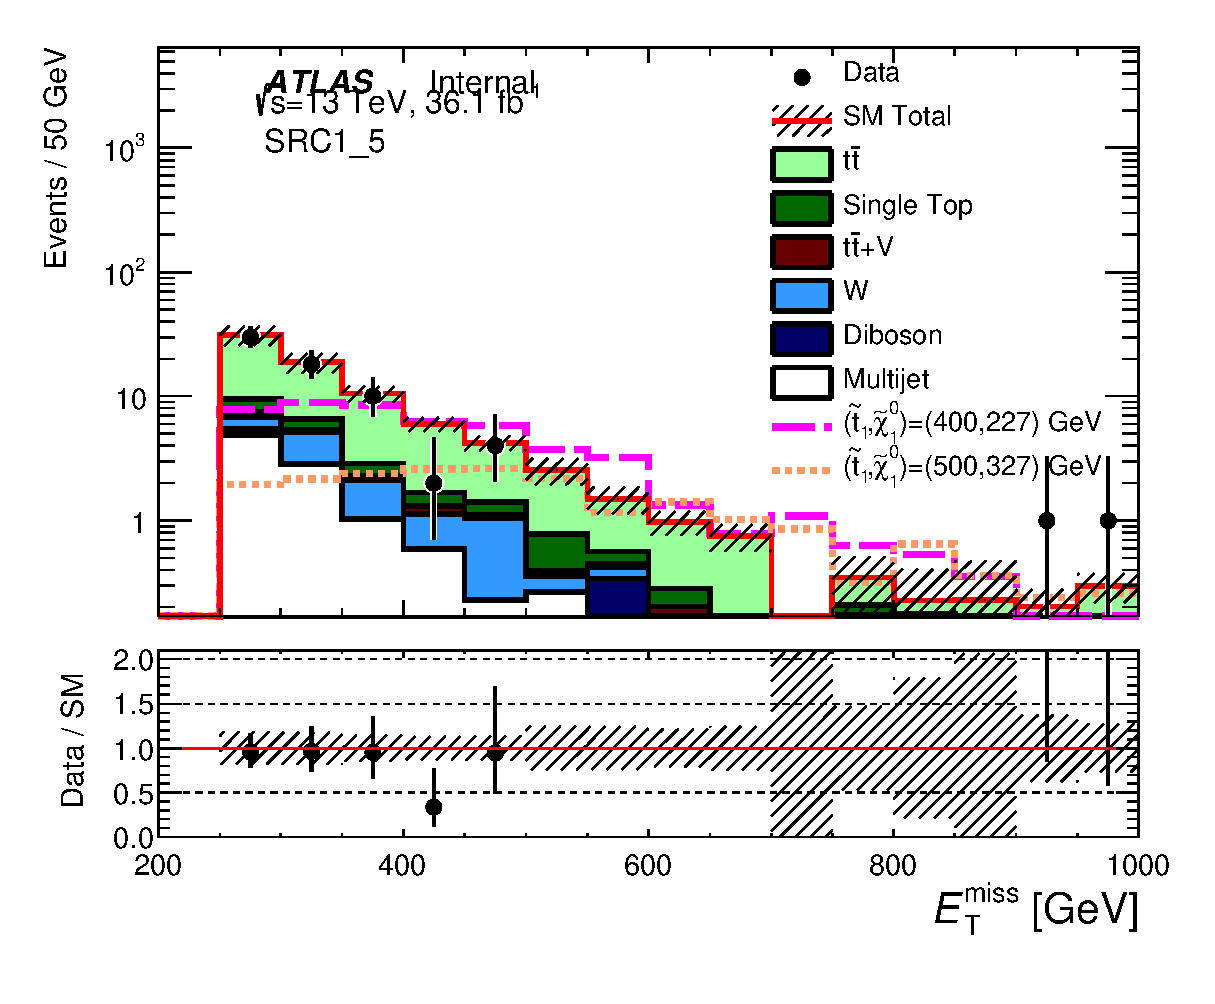
\includegraphics[width=\textwidth]{figures/plotRegion/Met_SRC1_5_log.eps}
                \caption{ }
    \end{subfigure}
        \begin{subfigure}[b]{0.40\textwidth}    
    	 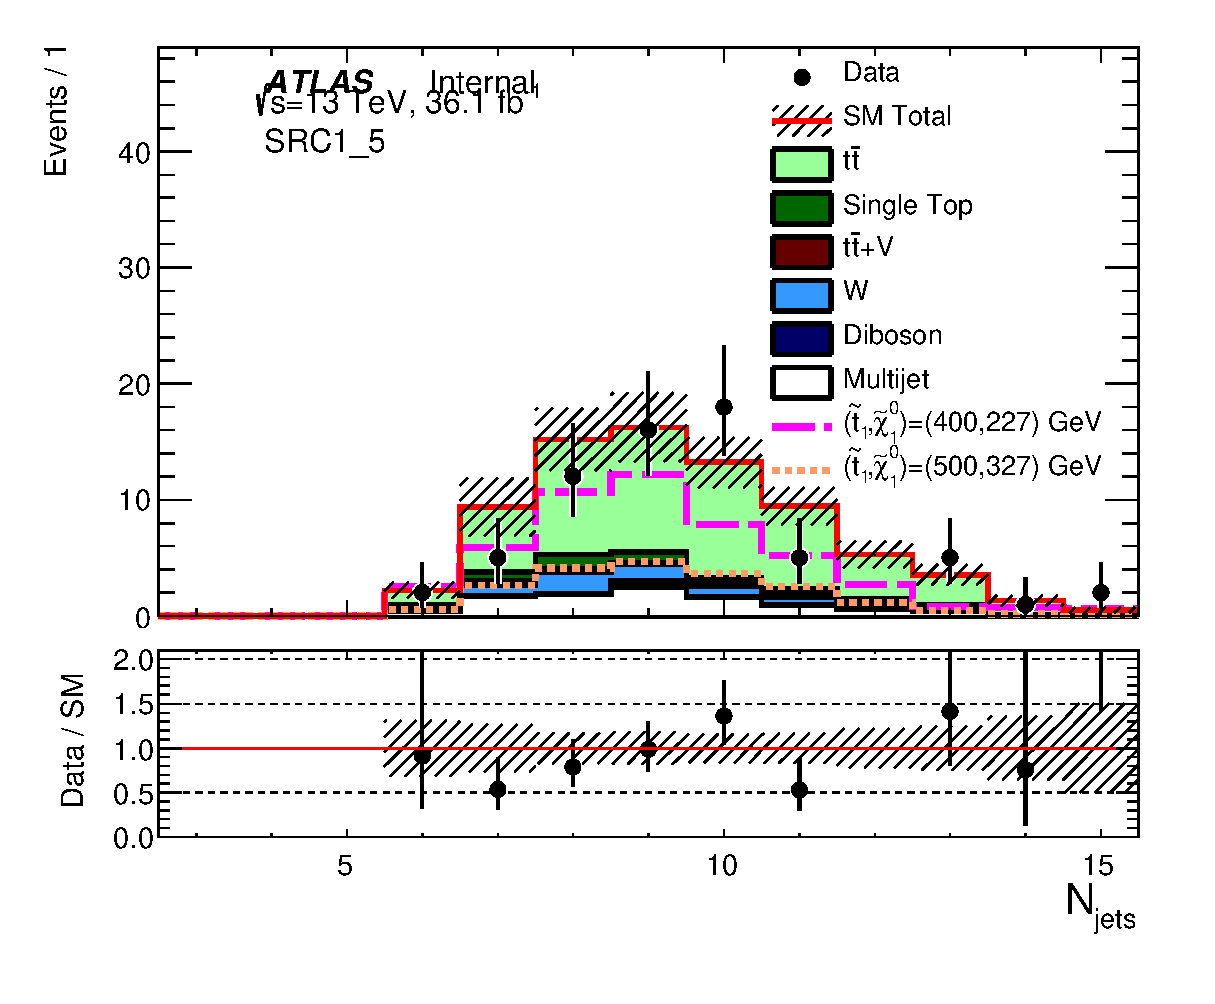
\includegraphics[width=\textwidth]{figures/plotRegion/NJets_SRC1_5.eps}
                \caption{ }
    \end{subfigure}
    \begin{subfigure}[b]{0.40\textwidth}    
    	 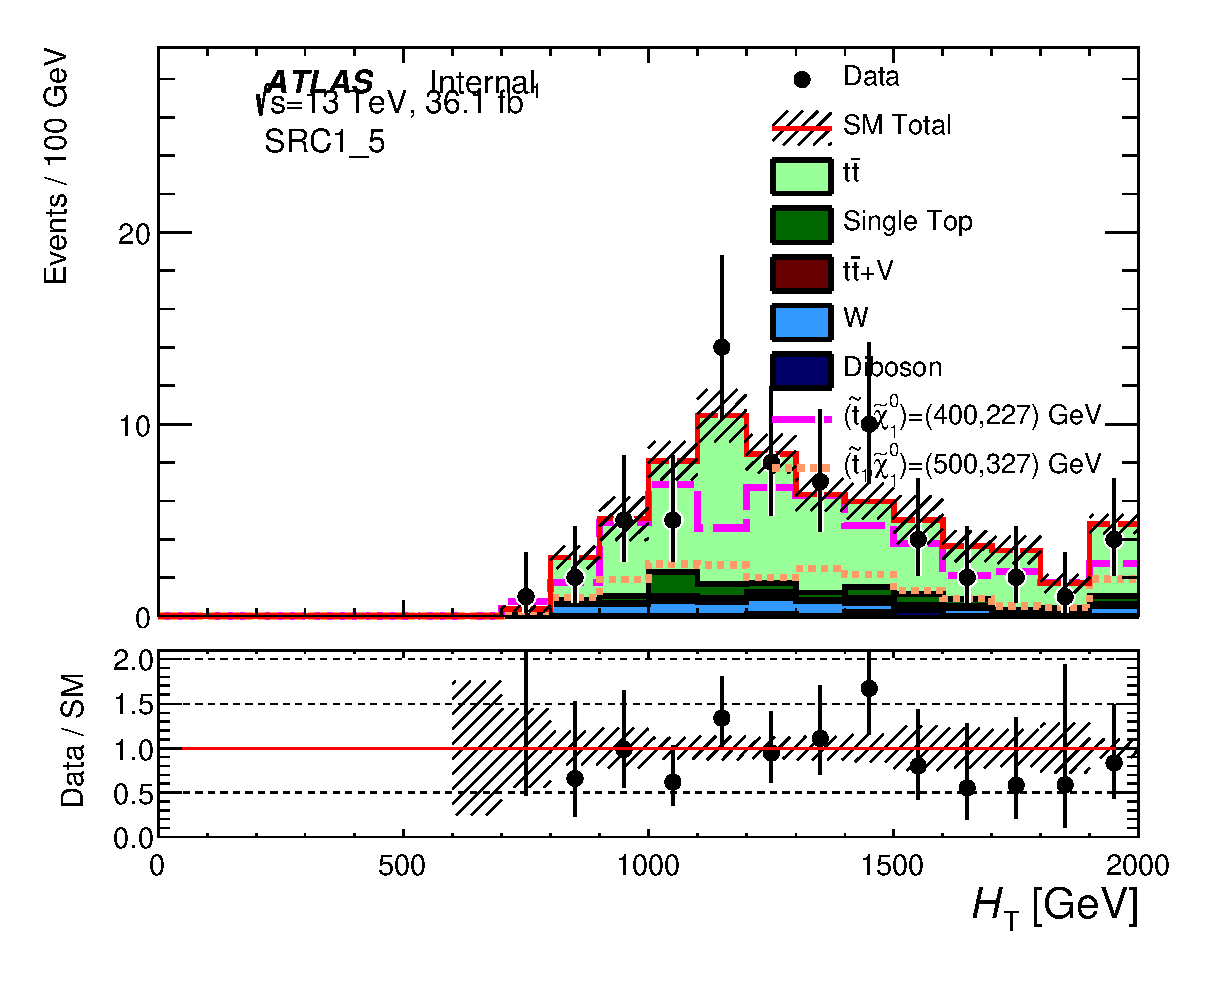
\includegraphics[width=\textwidth]{figures/plotRegion/Ht_SRC1_5.eps}
                \caption{ }
    \end{subfigure}
    \begin{subfigure}[b]{0.40\textwidth}    
    	 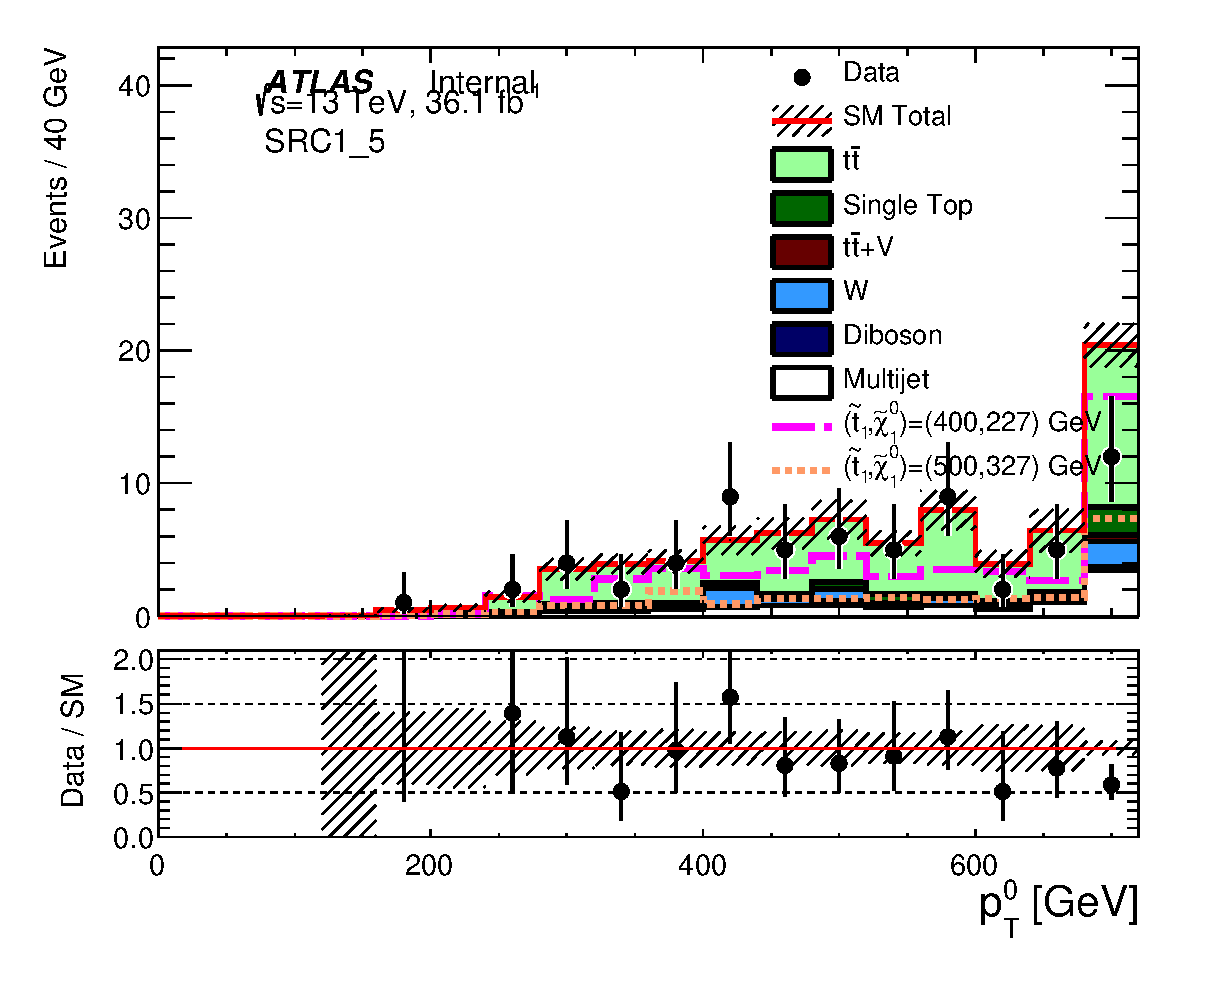
\includegraphics[width=\textwidth]{figures/plotRegion/JetPt_0__SRC1_5.eps}
                \caption{ }
    \end{subfigure}
    \begin{subfigure}[b]{0.40\textwidth}    
    	 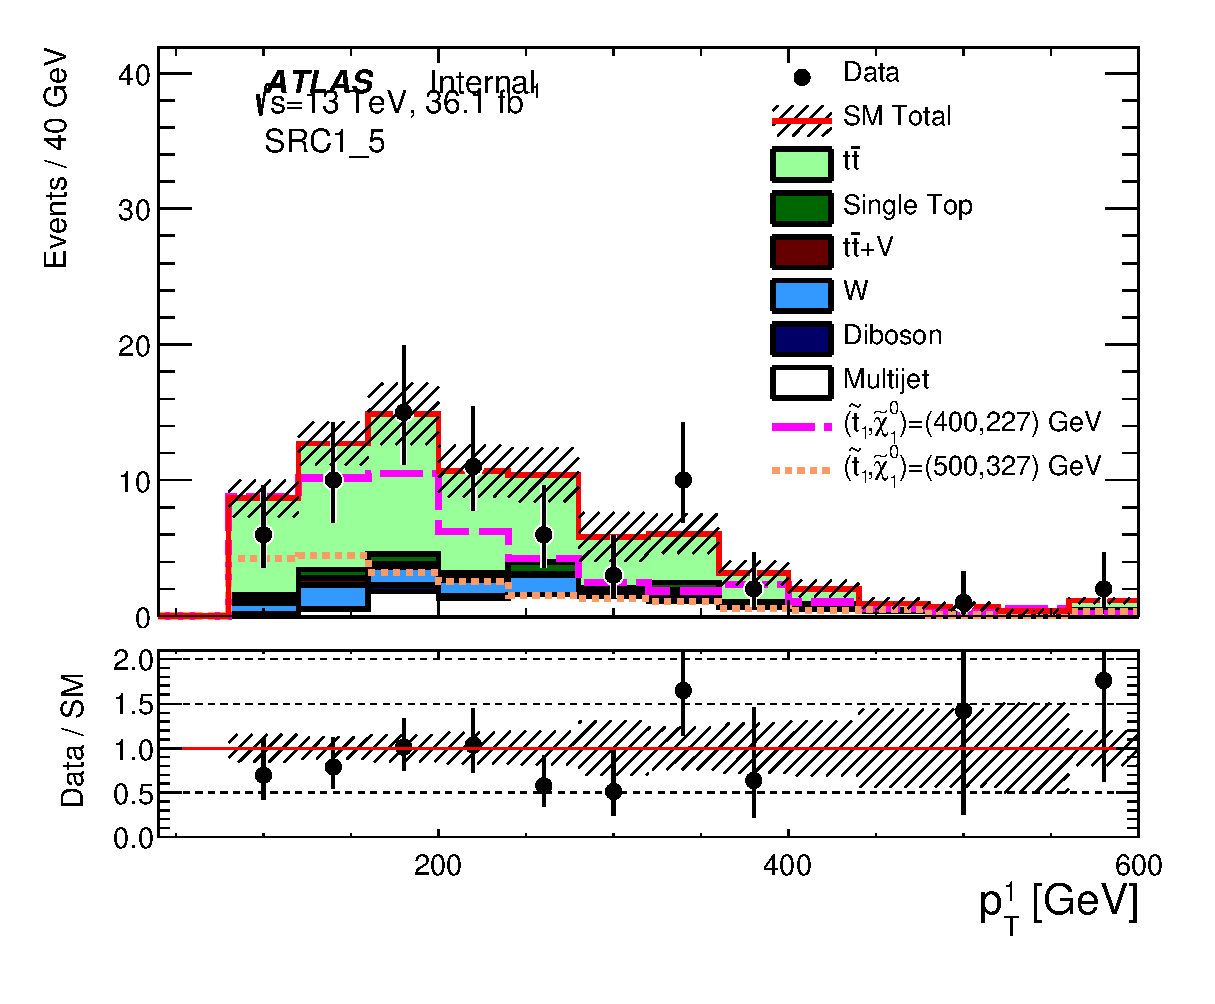
\includegraphics[width=\textwidth]{figures/plotRegion/JetPt_1__SRC1_5.eps}
                \caption{ }
    \end{subfigure}
    \begin{subfigure}[b]{0.40\textwidth}    
    	 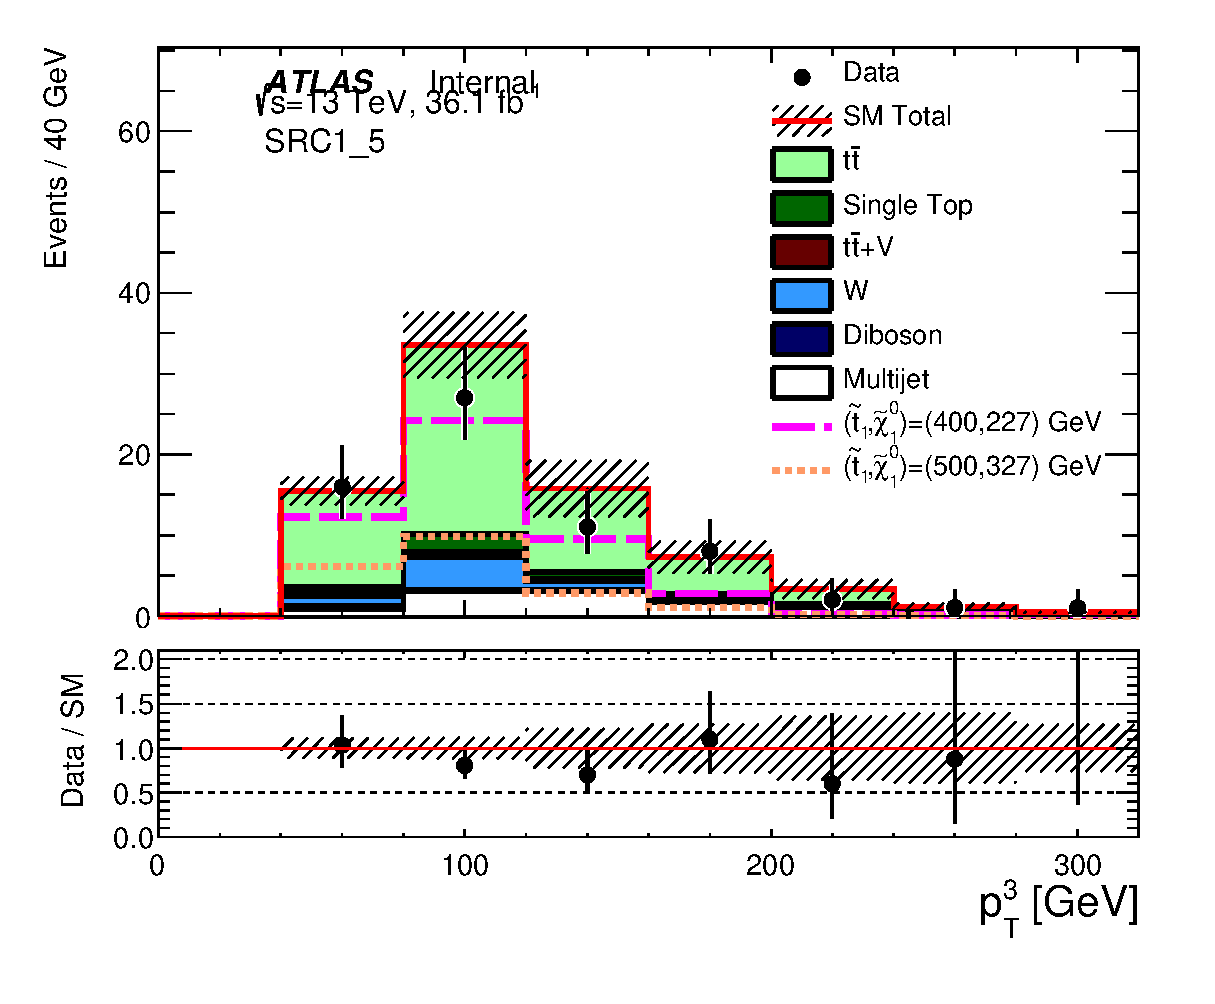
\includegraphics[width=\textwidth]{figures/plotRegion/JetPt_3__SRC1_5.eps}
               \caption{ }
    \end{subfigure}
     \caption[Distributions of kinematic variable after the signal region selection]{ Distributions of kinematic variable after the signal region selection; (a) $\met$ (b) number of jets (c) $\HT$ (d) $\pt$ of the highest $\pt$ jet (e) $\pt$ of the 2nd highest $\pt$ jet (f) $\pt$ of the 4th highest $\pt$ jet.  The solid stacked histogram represents the expected SM background rates. The dashed histogram represent the expected number of signal events for $m_{\stop} = 400,500$ \gev.  The hashed bars represent the size of the systematic uncertainty on the background.  The data/MC ratio is shown in the lower panel. }
  \label{fig:SR1}
    \end{center}
\end{figure}

\pagebreak

\begin{figure}[h!]
  \begin{center}
        \begin{subfigure}[b]{0.40\textwidth}    
    	 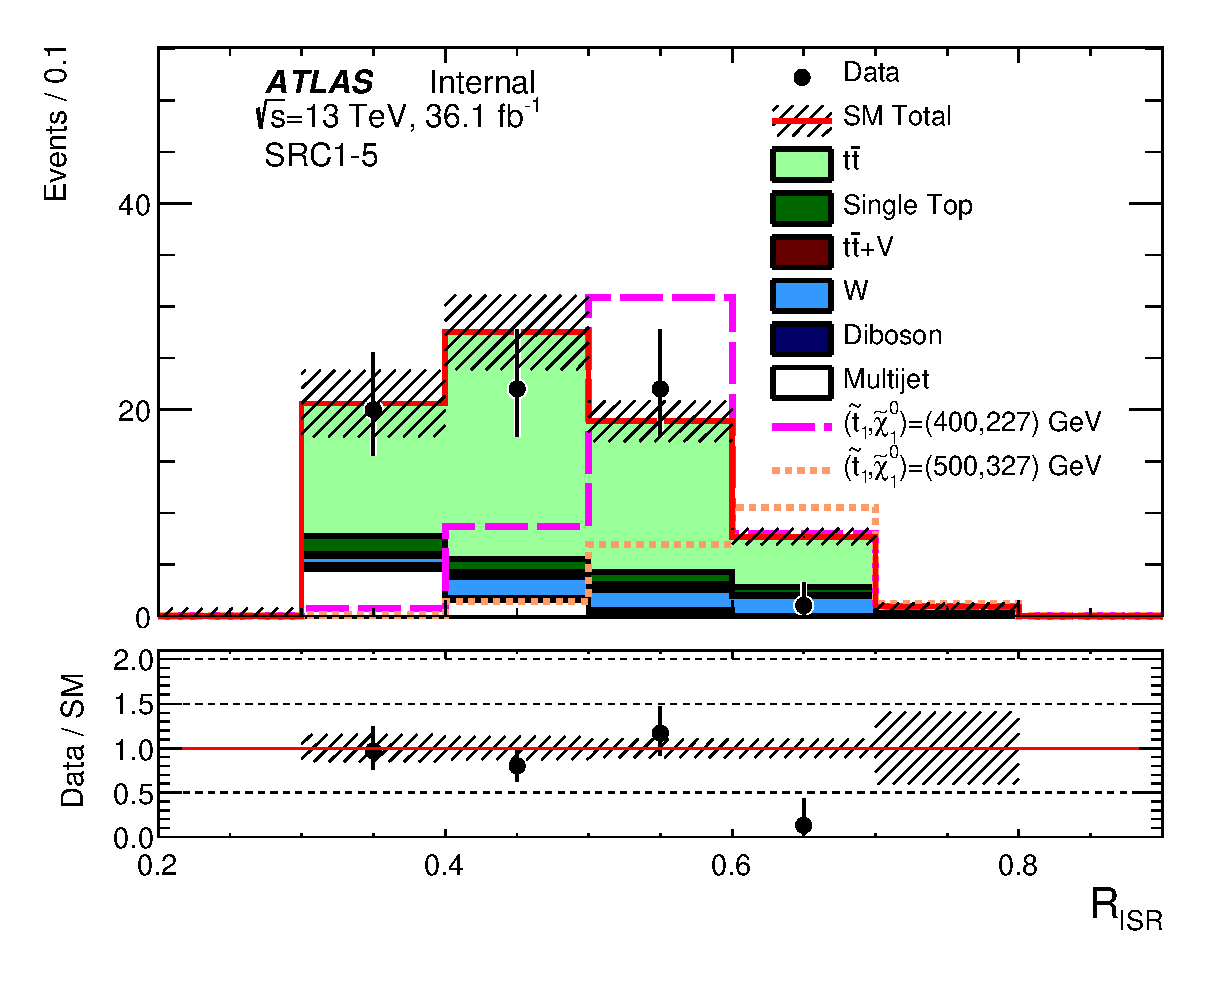
\includegraphics[width=\textwidth]{figures/SRC/CA_RISR_SRC1_5}
                \caption{ }
    \end{subfigure}
        \begin{subfigure}[b]{0.40\textwidth}    
    	 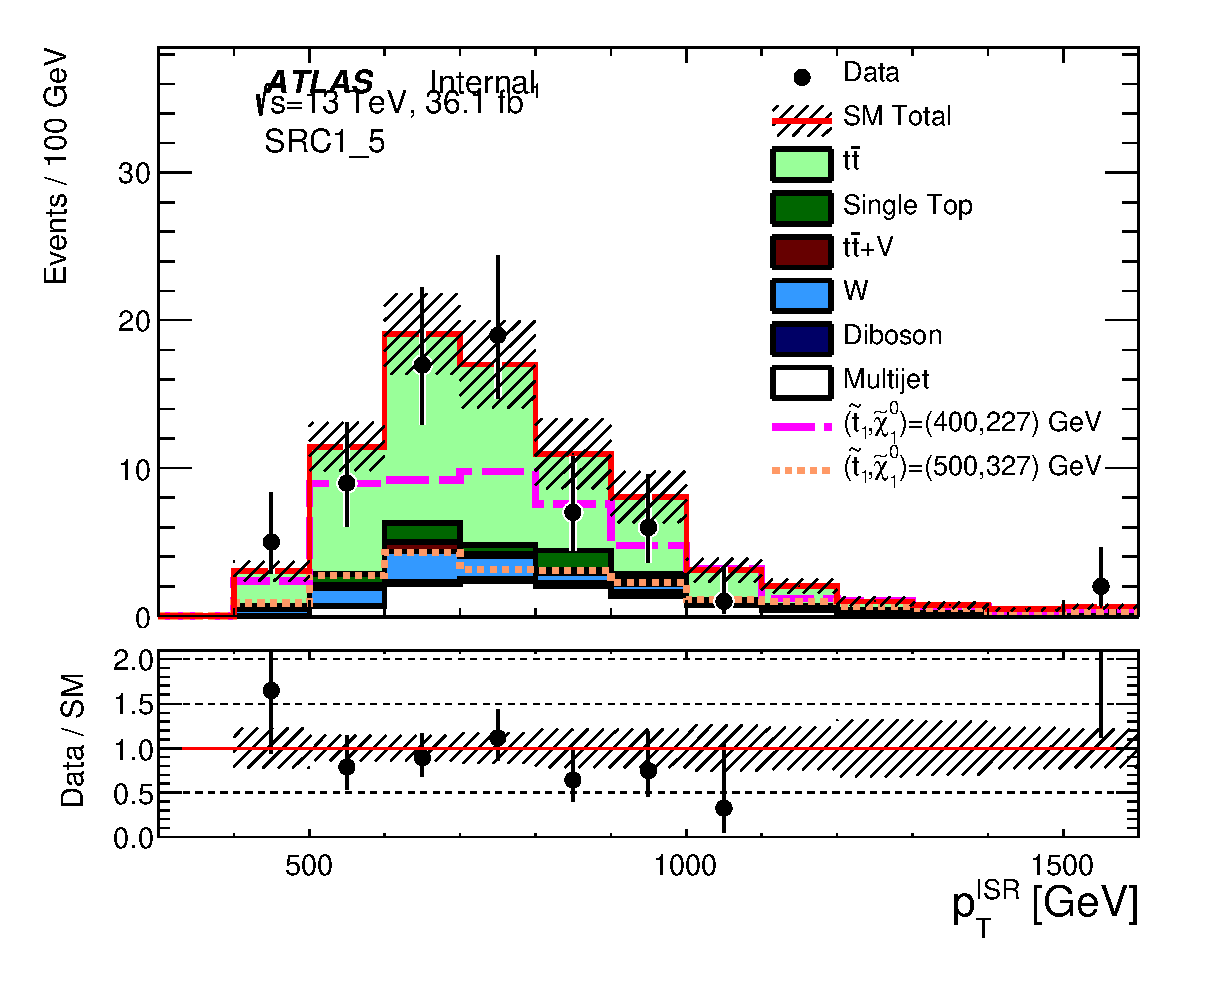
\includegraphics[width=\textwidth]{figures/plotRegion/CA_PTISR_SRC1_5.eps}
                \caption{ }
    \end{subfigure}
    \begin{subfigure}[b]{0.40\textwidth}    
    	 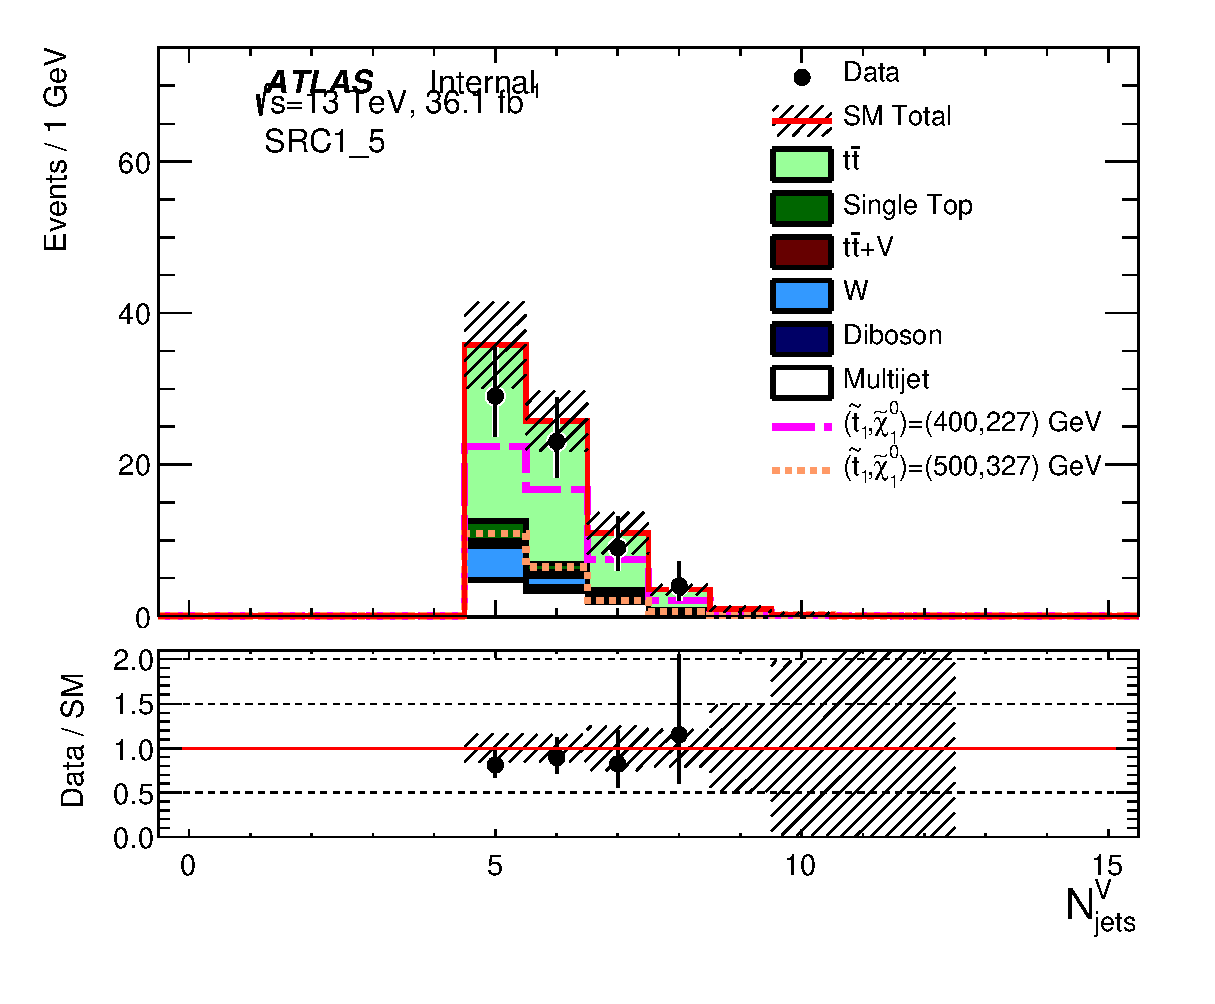
\includegraphics[width=\textwidth]{figures/plotRegion/CA_NjV_SRC1_5.eps}
                \caption{ }
    \end{subfigure}
    \begin{subfigure}[b]{0.40\textwidth}    
    	 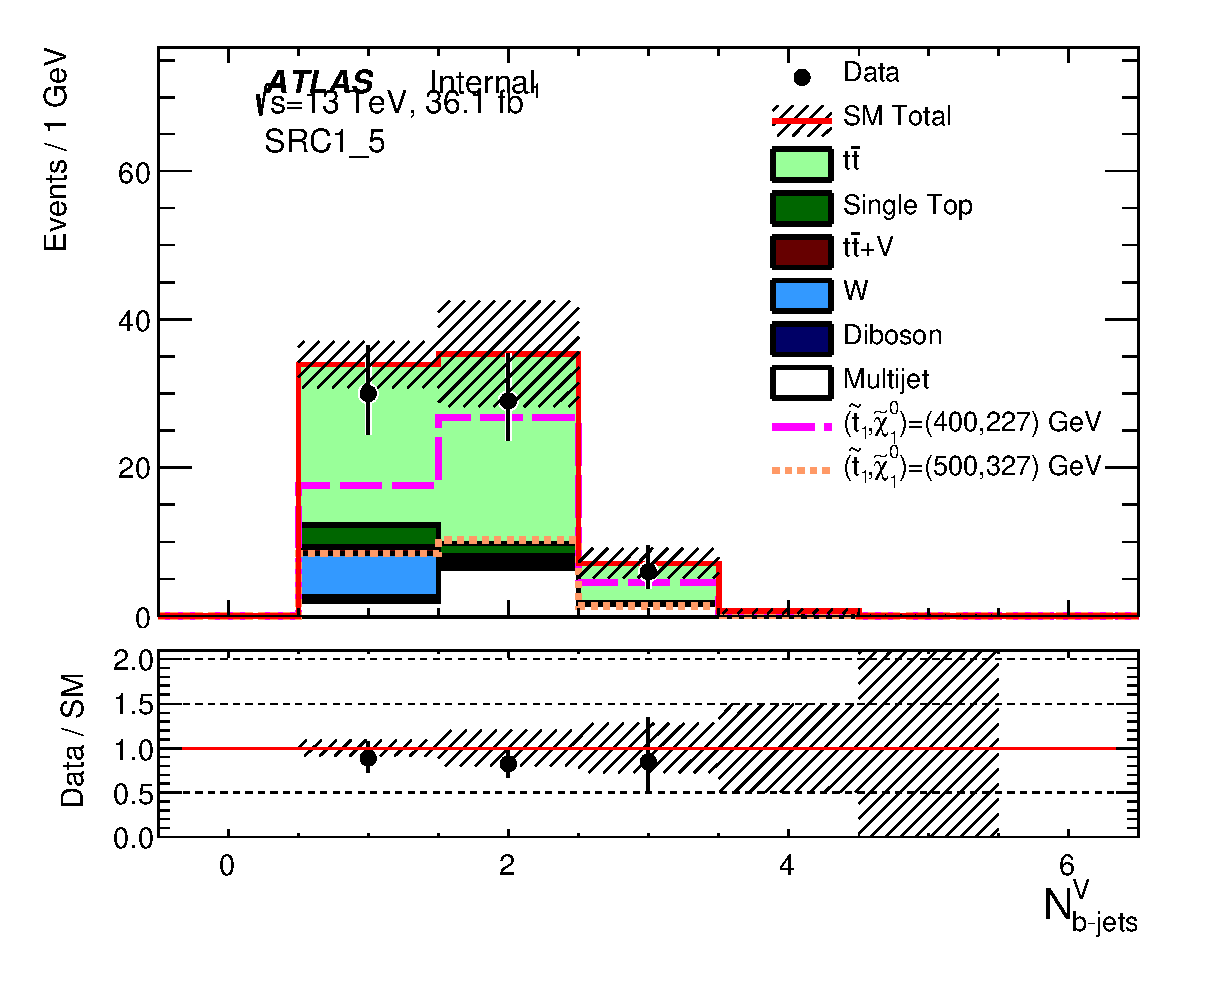
\includegraphics[width=\textwidth]{figures/plotRegion/CA_NbV_SRC1_5.eps}
                \caption{ }
    \end{subfigure}
    \begin{subfigure}[b]{0.40\textwidth}    
    	 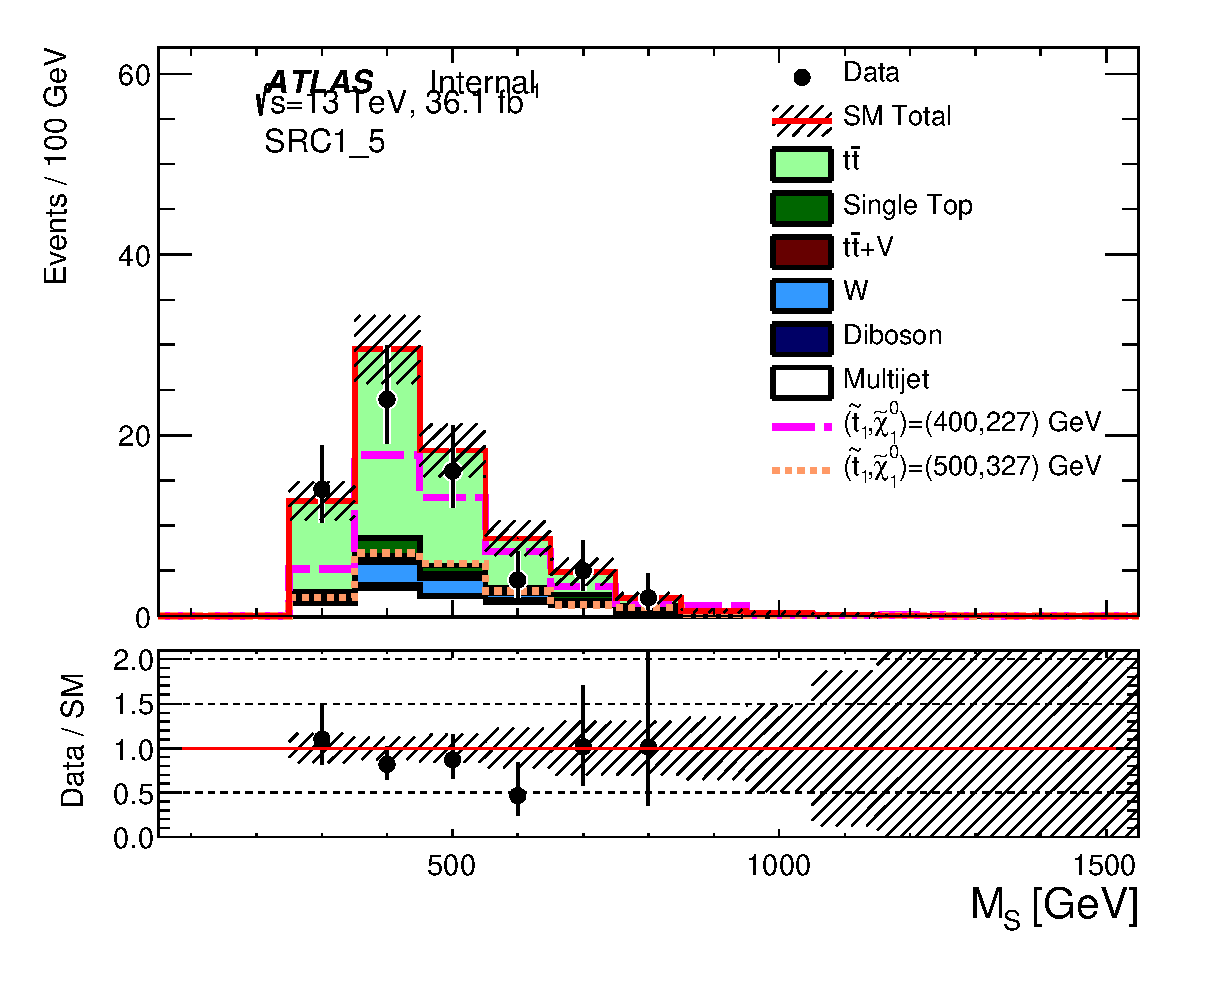
\includegraphics[width=\textwidth]{figures/plotRegion/CA_MS_SRC1_5.eps}
                \caption{ }
    \end{subfigure}
    \begin{subfigure}[b]{0.40\textwidth}    
    	 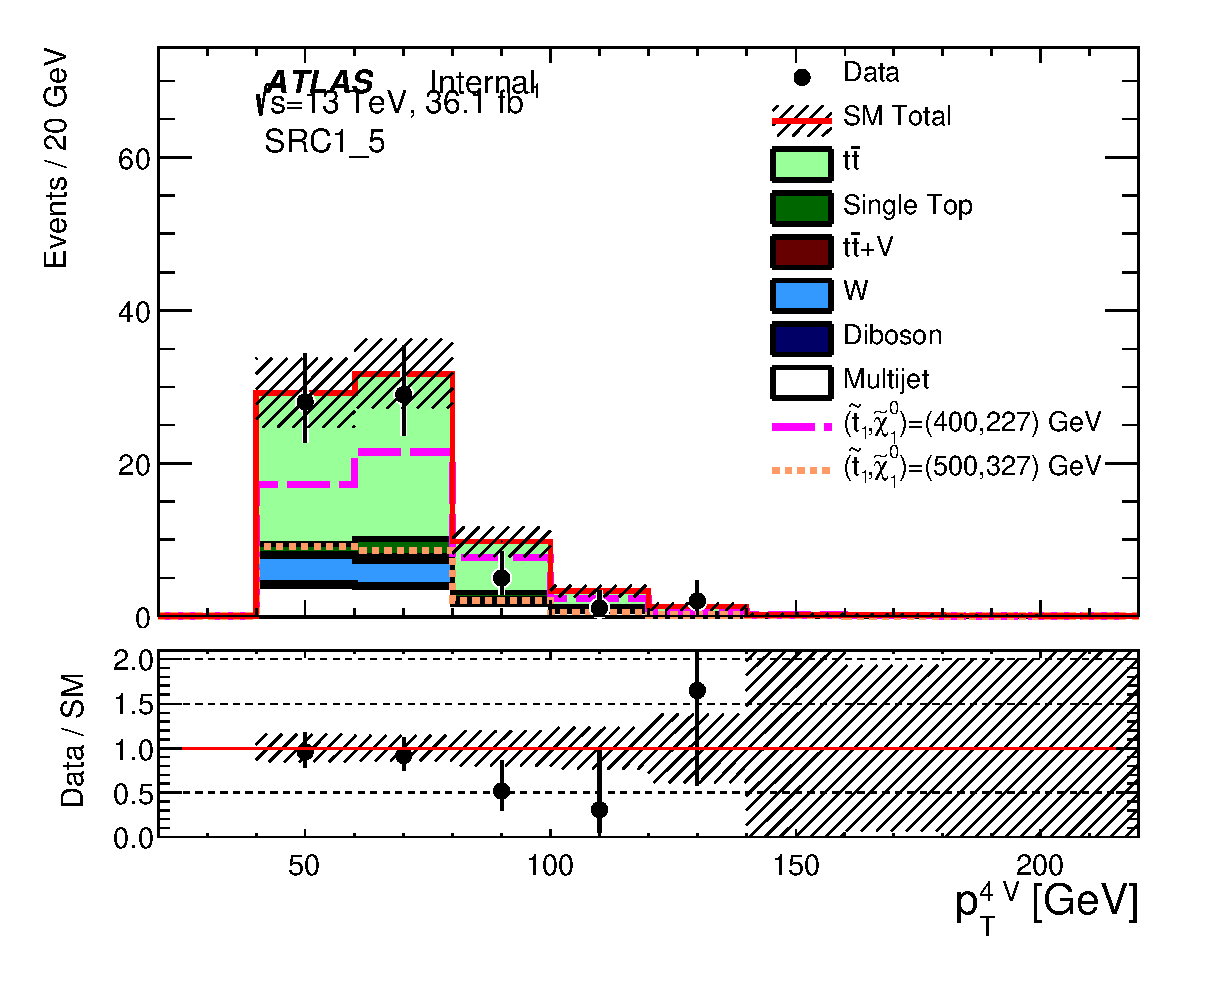
\includegraphics[width=\textwidth]{figures/plotRegion/CA_pTjV4_SRC1_5.eps}
               \caption{ }
    \end{subfigure}
     \caption[Distributions of kinematic variable after the signal region selection]{ Distributions of {\tt Recursive Jigsaw} kinematic variable after the signal region selection;  (a) $\RISR$  (b) $\PTISR$ (c) $\NjV$ (d) $\NbV$ (e) $\MS$ (f) $\pTjV$.  The solid stacked histogram represents the expected SM background rates. The dashed histogram represent the expected number of signal events for $m_{\stop} = 400,500$ \gev.  The hashed bars represent the size of the systematic uncertainty on the background.  The data/MC ratio is shown in the lower panel. }
  \label{fig:SR2}
  
   % 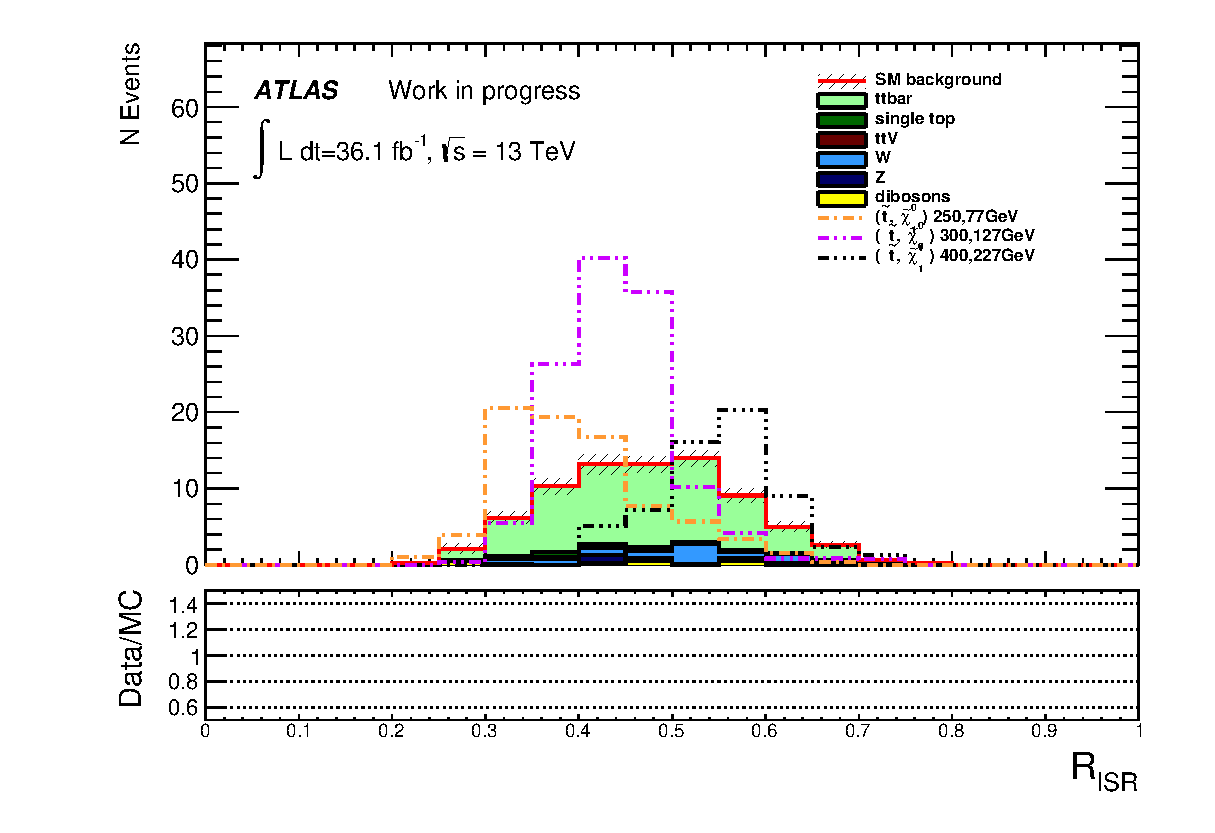
\includegraphics[width=0.45\textwidth]{figures/plotSR/SR_ND1_RISR_7SR.eps}
    %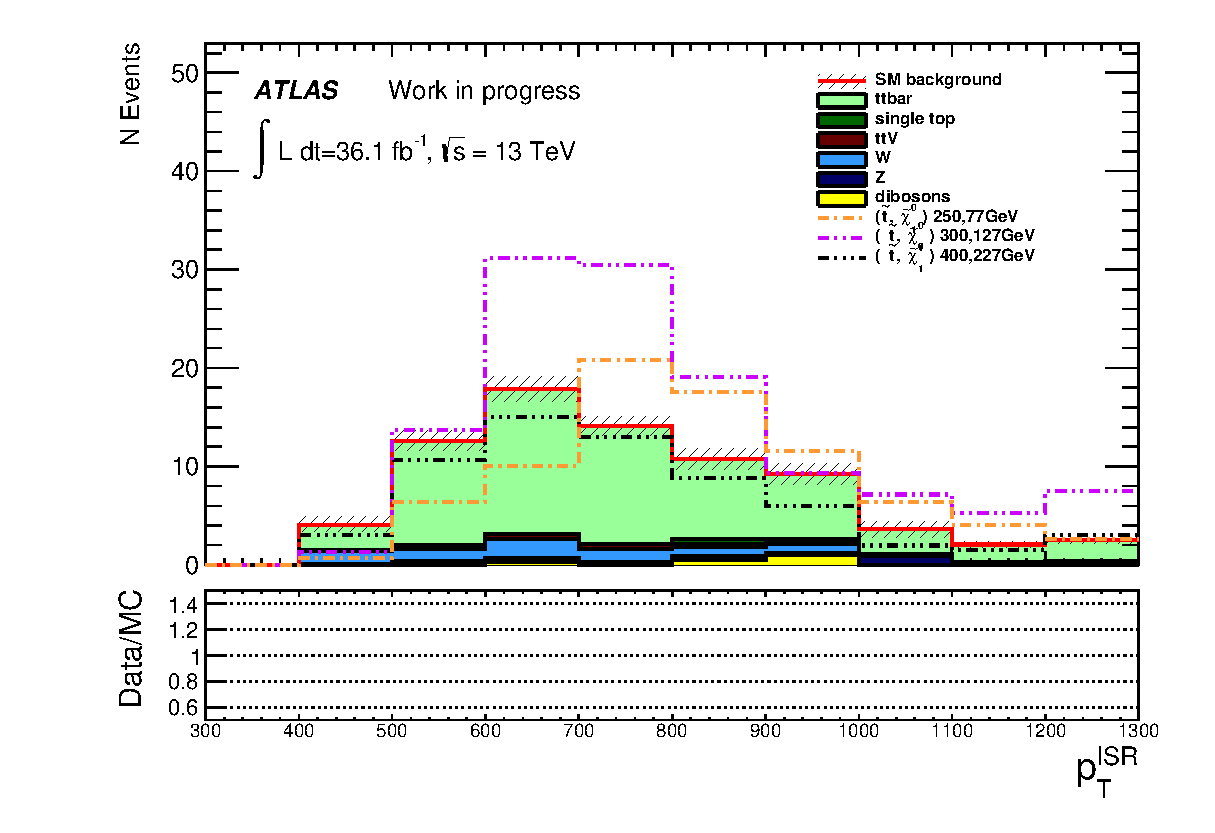
\includegraphics[width=0.45\textwidth]{figures/plotSR/SR_ND1_PTISR_7SR.eps}
    %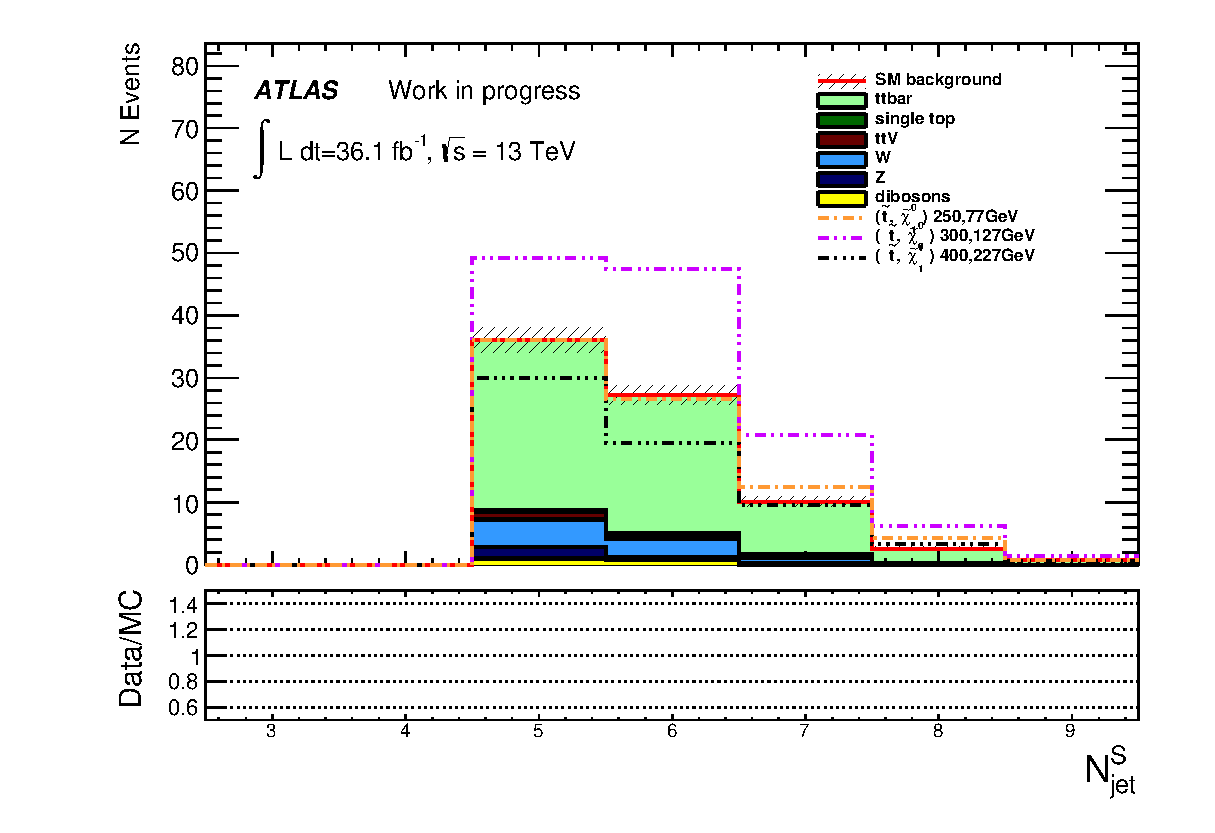
\includegraphics[width=0.45\textwidth]{figures/plotSR/SR_ND1_NjV_7SR.eps}
    %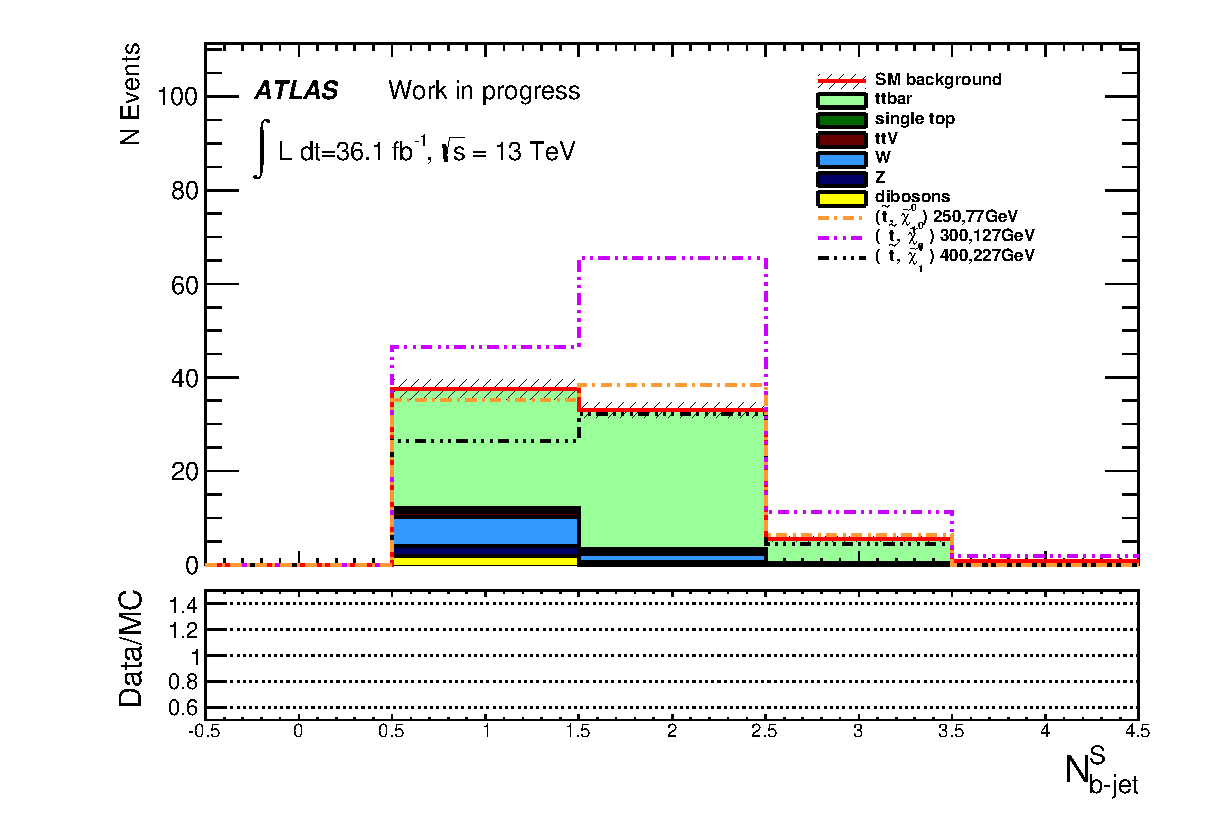
\includegraphics[width=0.45\textwidth]{figures/plotSR/SR_NbV_7SR.eps}
    %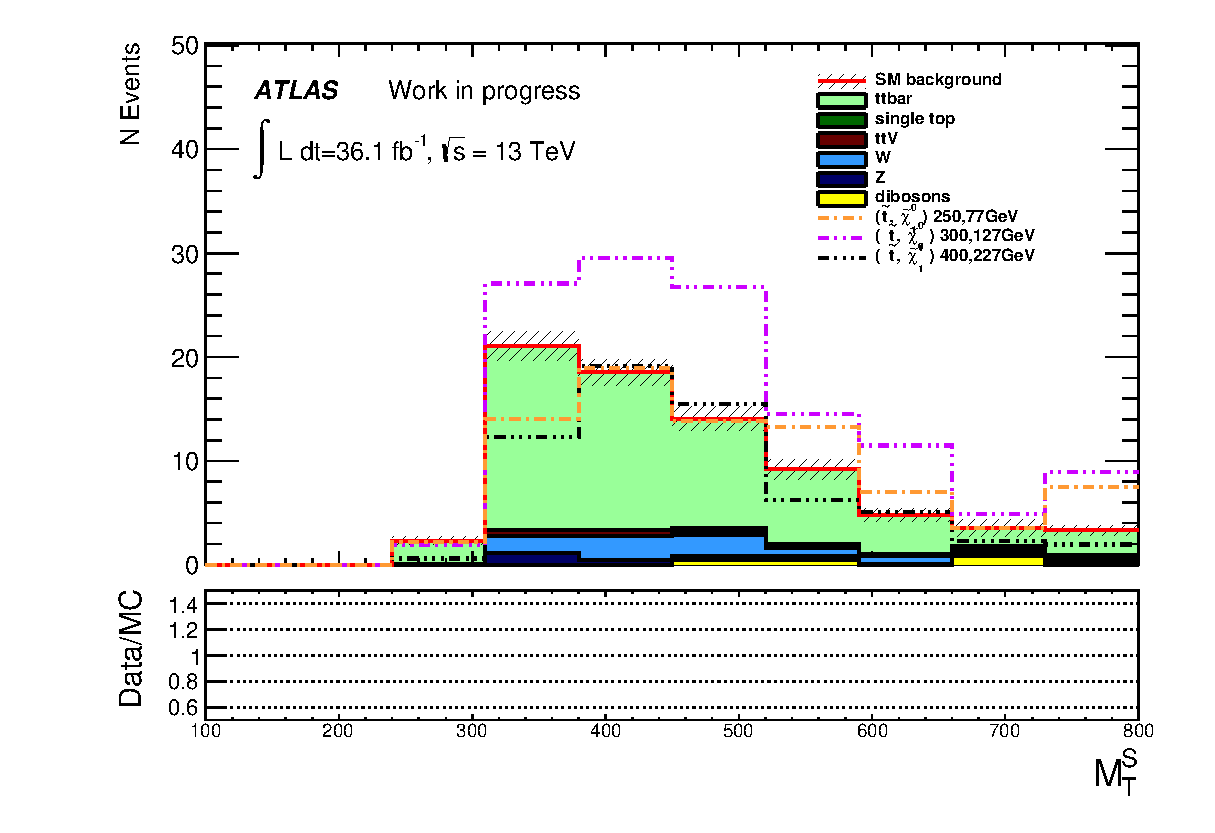
\includegraphics[width=0.45\textwidth]{figures/plotSR/SR_ND1_MS_7SR.eps}
    %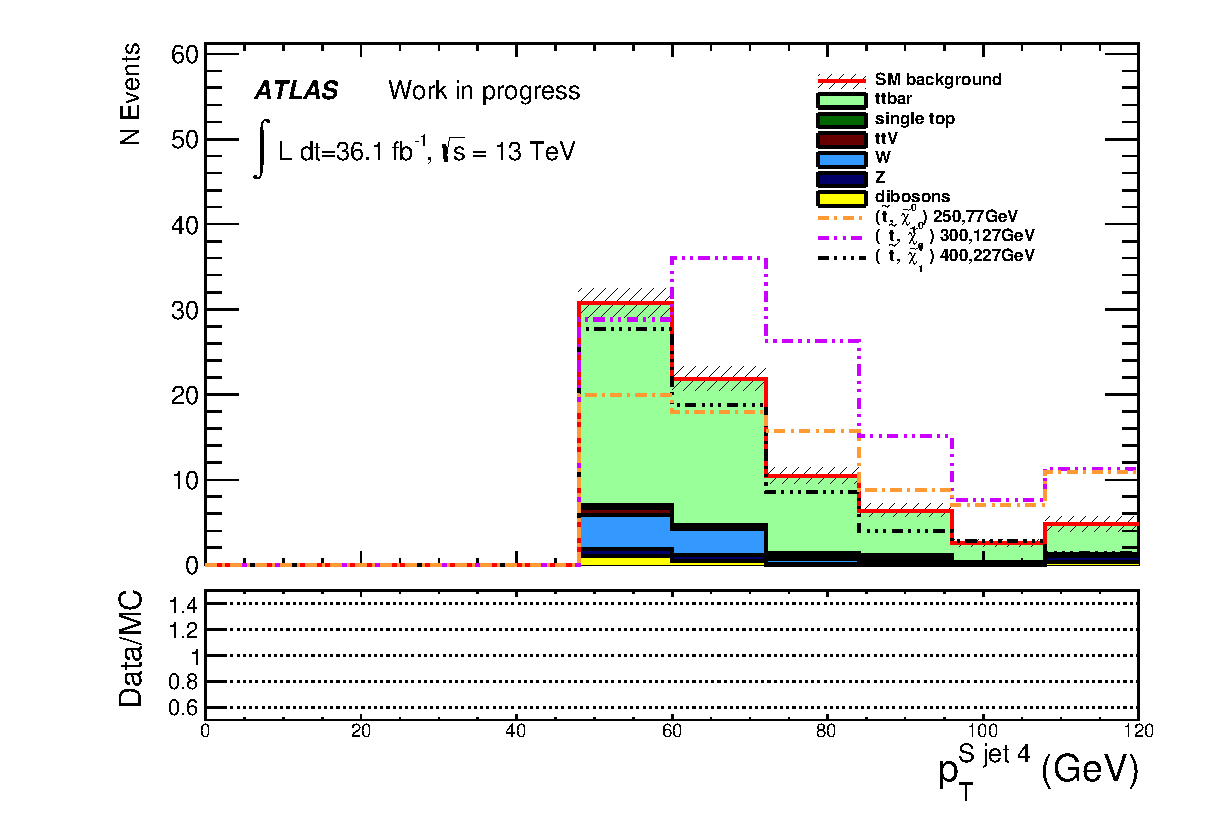
\includegraphics[width=0.45\textwidth]{figures/plotSR/SR_ND1_pTjV4_7SR.eps}
    %\caption[Kinematic distributions for signal region selection]{ Kinematic distributions for signal region selection. The hashed area in both the top and lower panel represent the uncertainty due to MC statistics.  QCD background estimation is not included.  }
  %\label{fig:SR2}
    \end{center}
\end{figure}



